\chapter{O CERN e Física Experimental de Altas Energias}
\label{cap:cern}
\glsresetall

O \gls{cern} é o maior laboratório de Física de Partículas do mundo, 
está situado na fronteira da Suíça com
a França, e conta com a colaboração de cientistas vindos 
de diversas regiões do mundo. Desde sua fundação em 1954, tem sido uma das referências de
avanços tecnológicos. Dentre seus feitos constam a construção do primeiro 
colisor de prótons-prótons (1971), a descoberta 
da corrente de neutrons (1973), dos bóssom Z e W (1983), 
e a invenção da \emph{Web} (1990) \cite{webCERN}. O acelerador de partículas mais ambicioso 
\cite{Intro_Standard,Beiser} já construído é o \gls{lhc}, o atual experimento do
\gls{cern}, onde espera-se que o maior de seus 
detectores, o \gls{atlas}, dê respostas a diversas questões da Física de Partículas
Elementares e da natureza do universo.

Este trabalho está inserido no ambiente de colaboração internacional do detector
\gls{atlas}. O propósito deste capítulo é descrever a base para o entendimento desse ambiente
e os ferramentais nele utilizados, entretanto alguns assuntos serão mais
aprofundados do que apenas o necessário para o entendimento básico, com o
intuito de mostrar que os experimentos \gls{lhc}/\gls{atlas} vão muito além 
da busca pelo bóssom de Higgs. Serão introduzidos o estudo de Física de Partículas
Elementares e o \glslink{mp}{Modelo Padrão} (Seção \ref{sec:fis_part}), 
o experimento \gls{lhc} (Seção~\ref{sec:lhc}), o detector
\gls{atlas} (Seção~\ref{sec:ATLAS}), tratando de seu sistema de calorimetria
(Seção~\ref{ssec:calorimetria}), assim como o ferramental utilizado pela colaboração
(Seção~\ref{sec:ferramentas}). 

\section{Introdução a Física das Partículas Elementares}
\label{sec:fis_part}

Dá-se o nome de Física de Partículas Elementares, ou simplesmente Física de
Partículas, ao estudo dos constituintes
elementares e da natureza do universo. Embora a noção de que a matéria é
composta por um conjunto de constituintes elementares tenha surgido em cerca de
430 a.C., por Demócritos \cite{democritos}, o seu estudo na ciência moderna teve inicio apenas 
no século 19, quando o elétron foi descoberto por Thompson \cite{thompson}.
Uma das grandes conquistas do século 20 foi o desenvolvimento do \gls{mp}.  

\newacronym[type=Abrev]{qed}{QED}{EletroDinâmica Quântica}

\subsection{O Modelo Padrão}
\label{ssec:mp}

Qualquer teoria de Física de Partículas Elementares precisa ser consistente com
a Relatividade Especial. A junção da Mecânica Quântica, Eletromagnetismo e
Relatividade Especial foi realizada através da Lei de Dirac e da Teoria de
Campo Quântico. A Teoria de Campo Quântico teve como seu primeiro triunfo a
\gls{qed}, que descreve a interação de elétrons com o campo
eletromagnético. 

O \gls{mp}, como o \gls{qed} nele contido, é uma teoria de
interação de campos. Ele descreve de maneira 
bem sucedida as relações entre
partículas elementares conhecidas pela ciência atual 
\cite{Intro_Nuclear} e as características de
três interações entre essas partículas:
eletromagnética, fraca e forte. A interação gravitacional é
desprezível na escala da Física de Partículas, onde a massa da partículas é da
ordem de $10^{-27}$ kg \cite{Intro_Standard}.

\newacronym[type=Abrev]{si}{SI}{Sistema Internacional de unidades e medidas}

As unidades normalmente utilizadas no estudo de Física de Partículas são fm para
distância (equivalente a $10^{-15}$ m), MeV, GeV ou TeV para massa ou energia, onde 1
eV (elétron-volt) é a energia necessária para aumentar o potencial elétrico de
um elétron em um volt, equivalente a $1,6\times10^{-19}$ J no \gls{si}, ou em unidades
de massa 1eV/$c^2$ = $1,78\times10^{-36}$ kg. A unidade para
área é o \emph{barn}, definida por 1 b = $10^{-28} m^2$, utilizada em
termos de mb ou fb \cite{Intro_Nuclear}.

São utilizados no \gls{mp} doze férmions, partículas elementares, divididas em dois grupos: os
léptons e os quarks. Existem três diferentes gerações, ou famílias, de férmions, cada uma com maior
massa e carga. Ainda, existem quatro outras partículas de campo das
interações, chamadas de bóssoms de campo.
A Figura \ref{fig:modelo_padrao} contêm as diferentes partículas que são
descritas pelo \gls{mp}, e seus respectivos números quânticos, como as massas de repouso em $GeV/c^2$, momento
angular ou rotação, em unidades de $\hbar$, e carga elétrica normalizadas em função da carga
do elétron, $e$, cerca de $1,6\times10^{-19}$ C. Note que todos os férmions
possuem rotação de $\frac{1}{2}$, enquanto para os bóssoms esse valor é de 1.

\begin{figure}[h!t]
\centering
\includegraphics[width=0.6\textwidth]{imagens/standart_model.png}
\caption{O Modelo Padrão de interação entre partículas elementares. Extraído de
\cite{tese_torres}.}
\label{fig:modelo_padrao}
\end{figure}

%\newacronym[type=Simb]{bossonfoton}{\ensuremath{\gamma}}{Fóton (bóssom)} 
%\newacronym[type=Simb]{bossonZ}{\ensuremath{Z}}{Bóssom Intermediário Z} 
%\newacronym[type=Simb]{bossonW}{\ensuremath{W}}{Bóssom Intermediário W} 
%\newacronym[type=Simb]{quarku}{\ensuremath{u}}{Quark \emph{up} (partícula elementar)} 
%\newacronym[type=Simb]{quarkd}{\ensuremath{d}}{Quark \emph{down} (partícula elementar)} 
%\newacronym[type=Simb]{quarkc}{\ensuremath{c}}{Quark \emph{charm} (partícula elementar)} 
%\newacronym[type=Simb]{quarks}{\ensuremath{s}}{Quark \emph{strange} (partícula elementar)} 
%\newacronym[type=Simb]{quarkt}{\ensuremath{t}}{Quark \emph{top} (partícula elementar)} 
%\newacronym[type=Simb]{quarkb}{\ensuremath{b}}{Quark \emph{bottom} (partícula elementar)} 
%\newacronym[type=Simb]{bossong}{\ensuremath{g}}{Gluón (bóssom)} 
%\newacronym[type=Simb]{neutrinoEletron}{\ensuremath{\nu_e}}{Neutrino do elétron (partícula elementar)} 
%\newacronym[type=Simb]{neutrinoMuon}{\ensuremath{\nu_{\mu}}}{Neutrino do múon (partícula elementar)} 
%\newacronym[type=Simb]{neutrinoTaon}{\ensuremath{\nu_{\tau}}}{Neutrino do táon (partícula elementar)} 
%\newacronym[type=Simb]{eletron}{\ensuremath{e^{-}}}{Elétron (partícula elementar)} 
%\newacronym[type=Simb]{muon}{\ensuremath{\mu}}{Múon (partícula elementar)} 
%\newacronym[type=Simb]{taon}{\ensuremath{\tau}}{Táon (partícula elementar)} 

Além dessas partículas elementares, a Lei de Dirac prevê a
existência de uma antipartícula para cada partícula carregada
com a mesma massa e rotação, mas cargas invertidas. 
Quando um par de partícula e antipartícula entram em contato,
ambas de massa $m$, acabam se aniquilando e liberando sua energia de repouso $2mc$ em fótons e outras
partículas. As antipartículas são representadas através de uma barra acima dos símbolos
das partículas, ou, no caso de partículas com índices de carga, 
apenas os sinais da carga são invertidos. 
A antipartícula do elétron tem o nome de pósitron, por motivos
históricos \cite{Intro_Standard,Intro_Nuclear}. Partículas 
eletricamente neutras também possuem antipartículas, e, em alguns casos,
podem ser suas próprias antipartículas.

\subsection{Os bóssoms e as interações fundamentais}
\label{ssec:bossoms}

As interações são comunicadas através dos bóssoms, partículas elementares
de campo das interações. Cada interação tem seu
bóssom característico: o gluôn (g): interação forte; o fóton $\gamma$: interação 
eletromagnética; e os bóssoms W e Z: interação fraca.  
Os bóssoms W e Z possuem respectivamente massa de aproximadamente
80 e 90 GeV. Esse fato limita o alcance da interação fraca a cerca $10^{-3}$ fm,
uma vez que uma partícula de massa M só pode existir como parte de um estado
intermediário por tempo $\hbar/Mc^2$, viajando uma distância não maior que
$\hbar/Mc$. O bóssom W possui carga elétrica, enquanto o bóssom Z é neutro, sendo sua própria antipartícula.
O gluôn e o fóton não possuem carga, assim como massa de repouso, de forma que é esperado alcance de
interação infinito para os campos portados por essas partículas. 
Contudo, diferente do campo eletromagnético, o campo de
gluôns é confinado a um alcance de 1 fm. 
Assim, para distâncias maiores a 1 fm, a interação eletromagnética é dominante,
enquanto para distâncias menores, as interações forte e fraca também ocorrem.

\begin{table}
\centering
\resizebox{\textwidth}{!}{
\begin{tabular}{ccccc}
\hline
\hline
\textbf{Interação} & \textbf{Partículas Afetadas} & \textbf{Alcance} &
\textbf{Intensidade Relativa} & \textbf{Bóssoms} \\
\hline
\hline
\multirow{2}{*}{Forte} & Quarks & \multirow{2}{*}{$~10^{-15}$ m} &
\multirow{2}{*}{1} & Gluôns  \\
 & Hádrons &  &  & Mésons  \\
\hline
Eletromagnética & Partículas carregadas & $\infty$ & $10^{-2}$ & Fótons
\\
\hline
Fraca & Quarks e Léptons & $~10^{-18}$ m & $10^{-3}$ & W e Z\\
\hline
Gravitacional & Todas & $\infty$ & $10^{-39}$ & Gráviton \\
\hline
\hline
\end{tabular}
}
\caption{As quatro interações fundamentais. A intensidade relativa se dá em
relação a interação forte. Adaptado de \cite{Beiser}.}
\label{tab:interacoes}
\end{table}

Conseguiu-se unir as interações eletromagnética e fraca, chamada de interação
eletrofraca. O problema da realização de tal conexão se deu ao fato dos
bóssoms da interação fraca terem massa, fato não ocorrido para o caso da
interação eletromagnética. Para realizar essa união se mostrou que, em um
estado primitivo, uma única interação era mediada pelos quatro bóssoms sem massa.
Através de um processo chamado quebra de simetria espontânea, três dos quatro
bóssoms adquiriram massa e viraram as partículas Z e W, com a consequente
redução no alcance de interação, enquanto o quarto bóssom continuou sem massa,
tendo como consequência o alcance infinito para a parte eletromagnética da
interação original \cite{Beiser}.

\newacronym[type=Simb]{hbar}{\ensuremath{\hbar}}{constante de Planck reduzida
(\ensuremath{\frac{h}{2\pi}})} 

Os físicos esperam adicionar a interação gravitacional
através da partícula gráviton, que deverá ter rotação equivalente a 2
unidades de $\hbar$ e massa nula, entretanto não há nenhuma evidência 
experimental a favor ou contra sua existência \cite{Beiser}.
A Tabela~\ref{tab:interacoes} contêm um resumo sobre as interações
fundamentais.

\subsection{Léptons}
\label{ssec:leptons}

Os léptons podem ser subdivididos em dois grupos, 
um com massa e carga elétrica, idêntica e unitária: elétron, múon e táon; 
e outro neutro em carga e massa reduzida, estando relacionados com os léptons
carregados: neutrino do elétron, neutrino do múon e neutrino do táon. Dos
léptons carregados, o múon e o táon só diferem dos elétrons na sua massa e no
seu tempo de vida finitos, sendo o elétron o único estável.
Experimentalmente observa-se que um lépton só pode mudar para outro do seu mesmo
subgrupo, assim como um lépton só pode ser criado ou destruído em conjunto com
um anti-lépton do mesmo subgrupo. Esse fato pode ser melhor observado no
decaimento descrito por \ref{eq:muon}, onde um múon decaí em um
elétron, lépton carregado, criando ao mesmo tempo um neutrino do múon e um
antineutrino do elétron, ambos do grupo de léptons neutrinos.
Nenhum dos léptons sofrem interações com os gluôns, portadores da interação forte.
No caso do subgrupo dos léptons neutrinos, eles também não interagem com a
interação eletromagnética (fótons), 
uma vez que não têm carga, só interagindo com a interação fraca e, por esse motivo,
são de difícil detecção \cite{Intro_Nuclear,Intro_Standard}.

\begin{equation} \label{eq:muon}
\mu^{-} \rightarrow \nu_{\mu} + e^- + \bar{\nu}_{e}
\end{equation}

\subsection{Quarks e hádrons}
\label{ssec:quarks}

Os quarks possuem tanto sabores, que lhes descreve as características de massa e
carga elétrica, quanto um equivalente de carga de interação
forte, distinguido em três cores de carga forte: vermelho, verde e azul. 
Para cada geração existe um par de sabores, onde um dos constituintes do par tem
carga elétrica positiva, correspondente a $\frac{2e}{3}$,
e outro negativa, igual a $\frac{-e}{3}$. São os possíveis sabores: \emph{up}
(u) e \emph{down} (d), \emph{charm} (c) e \emph{strange} (s), \emph{top} (t) e
\emph{bottom} (b). Os quarks sofrem influência de todas as interações descritas
pelo \gls{mp}.

\newacronym[type=Abrev]{qcd}{QCD}{CromoDinâmica Quântica}

Uma dificuldade da investigação experimental dos quarks é devida aos mesmos
nunca terem sido observados isoladamente. Eles estão sempre confinados em sistemas
compostos, que se estendem a uma distância de até 1 fm, alcance máximo da interação forte. 
A \gls{qcd} é modelada na \gls{qed}, mas alterando a carga elétrica pelas cores do quark, 
prevê como os quarks e gluôns interagem para formar os hádrons. Mesmo
em colisões de altas energias os quarks se agrupam rapidamente em hádrons,
formando jatos hadrônicos \cite{Intro_Nuclear}. Esse confinamento dos quarks ocorre 
porque a interação forte é similar a uma mola, quanto mais afastados, maior é a
força de atração entre os quarks. Mas se energia suficiente for adicionada,
ao invés de um quark se liberar dos outros no hádron, a energia excedente produz
um par de quark-antiquark \cite{Beiser}.
Se dá ao nome dos sistemas compostos por quarks e gluôns de
hádrons, sendo os bárions e mésons os sistemas mais simples conhecidos. 

%\newacronym[type=Simb]{kaon}{\ensuremath{K}}{Káon (méson)} 
%\newacronym[type=Simb]{pion}{\ensuremath{\pi}}{Píon (méson mais leve existente)} 
 
Um largo espectro dos bárions podem ser explicados como uma cápsula contendo
três quarks confinados por gluôns, sendo exemplos os prótons e nêutrons. Os mésons
são compostos essencialmente por um quark e anti-quark ligados
transientemente por um gluôns. Alguns dos mésons referidos neste trabalho são
os mésons mais leves existentes, os píons: $\pi^{+}$,
$\pi^{-}$ e $\pi^{0}$, compostos respectivamente por pares $u\bar{d}$, $\bar{u}d$ e
$u\bar{u}$ ou $d\bar{d}$, e os káons, os mais leves dos mésons estranhos
(contendo quarks $s$), $K^{+}$, $K^{0}$, $K^{0}_{S}$ e $K^{0}_{L}$, 
compostos pelos sistemas $u\bar{s}$, $d\bar{s}$,
$\frac{d\bar{s}+s\bar{d}}{\sqrt{2}}$, onde a diferença do $K^{0}_{S}$ e
$K^{0}_{L}$ está no tempo de vida médio dessas partículas. 
O próton ($uud$) é o único bárion estável\footnote{Teorias atuais consideram que
o próton decai com um tempo de vida muito longo, entretanto esse valor talvez seja maior 
que o valor mínimo detectado experimentalmente, de $10^{32}$ anos. 
Para comparação, a idade do universo é de $10^{10}$ anos \cite{Beiser}.}, 
já o nêutron ($udd$), apesar de estável na estrutura atômica,
quando isolado tem vida média de 15 minutos \cite{Intro_Standard}. Finalmente, 
todos mésons são instáveis e também são bóssoms, uma vez que mediam a interação
forte entre hádrons.

\subsection{A simetria e a física}
\label{ssec:simetria}

A construção do \gls{mp} foi guiada pelos princípios 
de simetria, que podem ser divididos em diversos grupos com diferentes
propriedades matemáticas. A conexão entre a física e simetria é forte, como
demonstrado pelo Teorema de Noether, onde essencialmente, para cada simetria
continua na natureza existe uma lei de conservação correspondente. De maneira
geral, a simetria de um tipo particular existe quando uma certa operação não
altera um certo fenômeno ou objeto. A operação de simetria mais simples é a
translação no espaço, que significa que as leis da física não dependem do local
das coordenadas de origem escolhidas. Noether mostrou que essa invariância tem a
consequência da conservação do momento linear. De forma semelhante a translação
no tempo, significando que não importa a escolha de $t = 0$, resulta na
conservação de energia e a invariância de rotações no espaço, ou seja, as leis
da física são invariantes conforme a escolha da orientação do sistemas de
coordenadas, resultam na conservação de momento angular
\cite{Intro_Standard,Feynman}.

\newacronym[type=Abrev]{cp}{CP}{Carga e Paridade}

Duas leis de conservação importantes na Física de
Partículas são: Conjugação de \gls{cp}, referidas como Simetria \gls{cp}. 
A Simetria \gls{cp} diz que a física deve reagir
da mesma maneira se a partícula for alterada para sua antipartícula (C) e refletida
espacialmente (P).
Embora a Simetria \gls{cp} seja conservada para as interações forte
e eletromagnética, o mesmo não acontece para a interação fraca
\cite{Intro_Nuclear}. Esse fato pode ser uma explicação possível do
desequilíbrio de matéria e antimatéria no universo, todavia, o \gls{mp} não
prevê a violação da Simetria \gls{cp} para as interações fracas, apenas para a
interação forte em escalas de energia muito altas, de forma que são necessárias
outras fontes de violação da Simetria \gls{cp} para se estudar e expandir o modelo.
 
\subsection{O bóssom de Higgs}
\label{ssec:higgs}

Outra simetria muito importante é conhecida como a Invariância de Gauge.
Ela prevê que todos os bóssoms de rotação unitária precisam ter
massa de repouso nula, se eles forem os únicos bóssoms da teoria.
Isso é aceitável para as teorias QED e QCD, uma vez que os
fótons e gluôns não possuem massa, mas é experimentalmente contraditório
para os bóssoms Z e W. A Invariância de Gauge tem um papel ainda mais forte
quando na teoria unificada eletrofraca, onde sua consequência é que todas as
partículas contêm massa nula. Foi introduzido um mecanismo, 
por Peter Higgs em 1964, para corrigir o \gls{mp} de modo que ele atendesse
a essa formulação, conhecido como o bóssom de Higgs, portador do campo de Higgs. O bóssom de Higgs seria
uma partícula mediadora responsável de fornecer massa às partículas elementares.

A existência do bóssom de Higgs é a mais importante previsão do \gls{mp} 
ainda não verificada experimentalmente e sua busca é de máxima importância para
a Física de Partículas. Diferente dos outros bóssoms, o
bóssom de Higgs teria rotação nula \cite{Intro_Nuclear}.

\subsection{A Física Experimental de Partículas}
\label{ssec:fisexp}

O progresso da ciência tem o comprometimento entre teoria e experimento. De
acordo com Kelvin, sem se medir ou poder expressar em números o assunto tratado, 
se há apenas uma ideia inicial do conhecimento sobre o tema \cite{kelvin}. 
Na Física de Partículas Elementares, experimentos atualmente dependem
principalmente de grandes aceleradores de partículas. Outras fontes de avanço na
Física de Partículas são experimentos com raios cósmicos, estudados tanto
através de detectores na superfície terrestre como através de satélites 
\cite{nature_space_and_time}. 

De acordo com a Teoria da Relatividade, não há diferença qualitativa entre
massa e energia, essa é apenas quantitativa \cite{einstein} sendo descrita por
\ref{eq:einstein}, onde $E$ é a energia, $m_0$ a massa de repouso, e $c$ a constante que representa a
velocidade de propagação da luz no vácuo, aproximadamente $3\times10^{8}$ m/s. Ao se acelerar
partículas de pequenas massas, é possível gerar partículas com maiores massas
através das interações ocorridas durante a colisão. Experimentos em
aceleradores de partículas tiveram seu início por volta de 1930, com o
acelerador linear \emph{Crockroft-Walton} em Cambridge, Reino Unido. Esse
acelerador atingia energias de 0,7 MeV com prótons. A Tabela~\ref{tab:aceleradores} 
lista alguns dos aceleradores já construídos. Os
aceleradores podem ser lineares ou circulares, assim como de alvo fixo ou colisores
de feixes. Nos aceleradores de alvo fixo as partículas são aceleradas até
obterem a energia desejada e então direcionadas a um alvo estacionário. Já nos
colisores de feixes, as partículas são aceleradas em feixes em direções
opostas e então colididas quando a energia desejada é atingida. A aceleração é
realizada através de interação eletromagnética, de forma que apenas
partículas carregadas eletricamente são aceleradas.

\newacronym[type=Simb]{E}{\ensuremath{E}}{energia} 
\newacronym[type=Simb]{massa}{\ensuremath{m}}{massa} 
\newacronym[type=Simb]{c}{\ensuremath{c}}{constante de velocidade de propagação da luz no
vácuo} 

\begin{equation} \label{eq:einstein}
E=m_0c^2
\end{equation}

\begin{table}
\centering
\begin{tabular}{lll}
\hline \hline \hline
\textbf{Máquina} & \textbf{Partículas Colididas} & \textbf{Início-Término} \\
\hline \hline
Tevatron & p: 900 GeV & 1987 \\
(Fermilab, Batavia, Ilinóia) & $\bar{p}$: 900 GeV & \\
\hline
SLC & $e^{+}$: 50 GeV & 1989-1998 \\
(SLAC, Standford) & $e^{-}$: 50 GeV & \\
\hline
HERA & e: 30 GeV & 1992 \\
(DESY, Hamburgo) & p: 820 GeV & \\
\hline
LEP2 & $e^{+}$: 81 GeV & 1996-2000 \\
(CERN, Genebra) & $e^{-}$: 81 GeV & \\
\hline
PEP-II & $e^{+}$: 9 GeV & 1999-2008 \\
(SLAC, Standford) & $e^{-}$: 3,1 GeV & \\
\hline
LHC & p: 7 TeV & 2008 \\
(CERN, Genebra) & p: 7 TeV & \\
\hline \hline
\end{tabular}
\caption{Alguns aceleradores de partículas no mundo. Adaptado de \cite{Intro_Standard}.}
\label{tab:aceleradores}
\end{table}

\newacronym[type=Abrev]{qgp}{QGP}{Plasma de Quarks e Glúons}

Muitos aceleradores de partículas utilizam prótons pois eles são mais facilmente
acelerados, atingindo níveis mais elevados de energia. Entretanto, a
estrutura dos prótons é muito mais complexa (hádrons
compostos por quarks e gluôns) que a dos elétrons (partícula elementar), de forma que as colisões com elétrons são 
de mais fácil compreensão. Como consequência, as
descobertas normalmente são realizadas através das colisões com prótons, enquanto as medições com
maior precisão são realizadas na colisão de elétrons \cite{nature_space_and_time}.
As colisões com íons de chumbo foram introduzidas em meados dos anos 80
para se estudar o \gls{qgp} \cite{heavy_ions}.

\subsection{Além do Modelo Padrão}
\label{ssec:alem_do_mp}

O \gls{mp} ainda deixa muitas questões em aberto. Não se foi capaz, até o
momento, de adicionar o campo gravitacional ao mesmo. São necessários a
determinação de cerca de 25 a 26 parâmetros quando considerando a existência do
bóssom de Higgs. Existem realmente tal ordem de parâmetros independentes na
natureza? Ainda, experimentos astronômicos mostram que apenas 4\% do universo é
composto pela matéria conhecida no \gls{mp}, outros 23\% são de Matéria
Escura, partículas ou conglomerados massivos que não brilham ou disseminam luz,
e os 73\% restantes, grande parte da energia do universo, são de Energia Escura,
totalmente desconhecida para a ciência atual. Indo mais além, o \gls{mp} 
não explica porque o universo se consiste quase totalmente por matéria e
praticamente nenhuma antimatéria, como foi dito quando se referindo a simetria
\gls{cp}. Espera-se que o experimento LHC seja capaz de responder a essas perguntas, entre outras, 
e ajude os cientistas a resolverem as incoerências e problemas do modelo, quem sabe também reduzindo 
o número de parâmetros livres a serem determinados para um, ou dois.
\cite{nature_space_and_time,Intro_Nuclear}

\newacronym[type=Abrev]{susy}{SUSY}{teoria de SUper-SImetria}
\newacronym[type=Abrev]{gut}{GUT}{Grande Interação Unificada}

Há ainda outras duas teorias além do \gls{mp}: a \gls{susy} e a Teoria de Cordas. 
A \gls{susy} é uma expansão do \gls{mp} com um
novo principio de simetria, no qual toda partícula deve ter uma contraparte
super-simétrica, chamadas de super-partículas. Dois aspectos da \gls{susy} são
que, em primeiro lugar, ela integra as teorias separadas do \gls{mp} para formar
um papel muito mais satisfatório na procura pela \gls{gut} -- união da interação
forte com a interação eletrofraca -- e, segundo, é concebível que a Matéria Escura 
é composta de super-partículas, ainda que não tenha sido observado nenhum sinal delas 
até o momento. 

A Teoria de Cordas tem o proposto de ser a Teoria de Tudo, que uniria a
gravidade com a \gls{gut}. Nessa teoria os léptons, quarks e bóssoms não são
pontos nas quatro dimensões (x,y,z,t) do espaço-tempo, mas laços vibrantes de
cordas em um espaço de dez dimensões. Cada partícula representa um módulo de
vibração, que tem $10^{-35} m$ e por isso supostamente se
assemelham a pontos. Não se há conhecimento das seis dimensões adicionais porque
elas estão "enroladas"~para nós da mesma forma que a analogia de um papel pode
parecer como uma linha unidimensional. A Teoria de Cordas, que é muito complexa
matematicamente, incorpora as principais características da \gls{gut}, incluindo,
em particular, a \gls{susy}.

\section{O \emph{Large Hadron Collider}}
\label{sec:lhc}

\glsreset{lhc}
\newacronym[type=Simb]{ionsChumbo}{A}{íons de chumbo} 
\newacronym[type=Simb]{protons}{p}{prótons} 

Atualmente, o \gls{cern} está engajado no projeto \gls{lhc}, 
um acelerador de partículas circular de 27 km de
circunferência, situado no subsolo, dentre 50 e 175 m, custando \euro $3,03
Bi$ \cite{webLHC}. Sua parte central é um dos pontos mais frios do universo,
operando a 2 K, temperatura menor que a temperatura média do espaço. Ainda, o
vácuo desenvolvido nos seus tubos de feixes ($10^{-13}$ atm) é o espaço mais vazio do Sistema
Solar \cite{closerLook}. A potência necessária para abastecer o experimento por
completo é de 180 MW, sendo estimados um consumo total de 700 GWh durante o
ano de 2009 \cite{webLHC}. 

No presente momento, ele realiza colisões de pacotes contendo $1,5\times10^{11}$ \gls{protons} 
a uma energia de 7 TeV no centro de massa, que serão expandidos a 14 TeV em 2013
\cite{webATLAS}. Para desenvolver essa energia a velocidade dos prótons será de 
$0,999999991\acrshort{c}$, percorrendo o \gls{lhc} 11000 vezes por segundo.
O \gls{lhc} também colidirá \gls{ionsChumbo}, num total de 5,5 TeV para cada par
de núcleons.

\subsection{Os objetivos do LHC}
\label{ssec:obj_lhc}

O \gls{lhc} apresenta uma oportunidade sem precedentes para conhecer os domínios da
nova física na região TeV e lançar luz sobre algumas das questões fundamentais
não resolvidas da Física das Partículas Elementares.
No caso das colisões de p-p, dentre os tópicos principais a serem testados pelo
\gls{lhc} estão \cite{hunt_for_physics}:

\newacronym[type=Abrev]{hs}{HS}{Setor Escondido}
\newacronym[type=Simb]{zprime}{Z'}{Z \emph{prime}}

\begin{itemize}
\item \textbf{Busca pelo bóssom de Higgs}: Tópico no qual este trabalho está
inserido. Se tal partícula existir, o \gls{lhc} deverá ser capaz de observá-lo;
\item \textbf{Busca pela \gls{susy}}: Algumas partículas previstas por esse
modelo, as super-partículas, 
devem ser visualizadas na região TeV;
\item \textbf{Violação \gls{cp}}: Estudo da violação da Simetria \gls{cp};
\item \textbf{Matéria escura}: Os candidatos mais relevantes vão além do \gls{mp}
para descrever a matéria escura. Um dos possíveis modelos é a \gls{susy};
\item \textbf{Física do quark \emph{top}}: Busca melhorar a compreensão da física dessa
partícula elementar, ainda não muito bem compreendida;
\item \textbf{Física do \gls{zprime}}: Estudos dos possíveis bóssoms Z adicionais; 
\item \textbf{Assinaturas visiveis do \gls{hs}}: Modelos baseados em
cordas e membranas provêm um novo setor de física, o \gls{hs}, que poderá ser
explorado pelo \gls{lhc};
\item \textbf{Provar a origem da massa dos léptons neutrinos}: Se o mecanismo que gera
suas massas estiver na região TeV, o \gls{lhc} poderá resolver essa questão;
\item \textbf{Caça por dimensões extras}: Modelo com ordens superiores de dimensões
oferecem alternativas para a \gls{susy};
\item \textbf{Busca por cordas no \gls{lhc}}: A Teria de Cordas oferece a possibilidade de
união de todas as interações conhecidas na natureza, incluindo a gravidade. Muitos
trabalhos apresentados mostram predições de cordas na escala TeV.
\end{itemize}

\subsection{A estrutura e funcionamento do LHC}
\label{ssec:struct_lhc}

\newacronym[type=Abrev]{booster}{BOOSTER}{\emph{proton synchroton BOOSTER}}
\newacronym[type=Abrev]{ps}{PS}{\emph{Proton Synchroton}}
\newacronym[type=Abrev]{sps}{SPS}{\emph{Super Proton Synchroton}}
\newacronym[type=Abrev]{linac}{LINAC}{ACelerador LINear}

Para desenvolver a altíssima energia necessária para o experimento, o \gls{cern}
utiliza outros aceleradores construídos anteriormente, acelerando
sequencialmente os pacotes de hádrons até atenderem
a energia desejada para a colisão. Na Figura \ref{fig:esquema_aceleradores} pode-se observar
o esquema de aceleração, tanto para prótons, quanto para íons de chumbo. 
No caso dos prótons, o ciclo inicia-se na extração de prótons de átomos
de hidrogênio que são acelerados no \acrshort{linac} 2, um acelerador linear,
que inicia a sequencia de aceleração, proporcionando-lhes uma energia de até 50 MeV. 
Em seguida são utilizados síncrotons, aceleradores circulares no qual as
partículas seguem a trajetórias circulares dirigidas por magnetos: \acrshort{booster} (1.4
GeV), \acrshort{ps} (25 GeV), \acrshort{sps} (450 GeV), até finalmente 
abastecer o \gls{lhc} com os pacotes de prótons. O \gls{lhc} também é um
síncroton, assim como grande parte dos aceleradores de altas energias anteriormente 
construídos \cite{lecture_slides_1,lecture_slides_2}.

\begin{figure}[h!t]
\centering
\includegraphics[width=\textwidth]{imagens/lhc_garrafa_linac2.pdf}
\caption{Os diferentes aceleradores e detectores do CERN, extraído de
\cite{cern_accelerators}. A seta cinza claro corresponde ao sentido do
deslocamento de prótons nos aceleradores. A esquerda, foto da garrafa
de hidrogênio de onde são retirados os prótons, e na direita foto do LINAC 2.}
\label{fig:esquema_aceleradores}
\end{figure}

\newacronym[type=Abrev]{alice}{ALICE}{\emph{A Large Ion Collider Experiment}}
\newacronym[type=Abrev]{lhcb}{LHCb}{\emph{Large Hadron Collider beauty experiment}}
\newacronym[type=Abrev]{totem}{TOTEM}{\emph{Total Cross Section, Elastic
Scattering and Diffraction Dissociation}}
\newacronym[type=Abrev]{cms}{CMS}{\emph{Compact Muon Sollenoid}}
\newacronym[type=Abrev]{moedal}{MoEDAL}{\emph{the Monopole and Exotics Detector At the
\acrshort{lhc}}}
\newacronym[type=Abrev]{lhcf}{LHCf}{\emph{\acrshort{lhc} forward}}

\newacronym[type=Abrev]{fodo}{FODO}{\emph{FOcusing DefOcusing}}
\newacronym[type=Abrev]{rf}{RF}{\emph{Radio Frequency}}
\newacronym[type=Abrev,\glslongpluralkey={Pontos de Inserção},
\glsshortpluralkey={IPs}]{ip}{IP}{Ponto de Inserção}

O \gls{lhc} não é uma circunferência perfeita, sendo dividido em octantes, 
contendo dois arcos e um trecho reto, que se iniciam e termim no ponto
intermediário de arcos sucessivos. Os arcos medem cerca de 2,45 km,
cotendo 23 células em estrutura \gls{fodo}, que serão detalhadas
posteriormente nesta Seção. 
Cada trecho reto tem 528 m e são utilizados como \glspl{ip},
seja para um experimento ou para uma utilidade. A parte
compreendida entre dois \glspl{ip} é chamada de setor. A 
Figura~\ref{fig:esquema_lhc} contêm um esboço da estrutura do \gls{lhc}, assim
como as utilizações de seus \glspl{ip}.

\begin{figure}[h!t]
\centering
\includegraphics[width=.6\textwidth]{imagens/lhc-schematic.png}
\caption{Esboço esquemático do LHC, extraído de
\cite{webLHC}. Os diversos octantes do LHC, contendo os pontos de inserção 
com suas respectivas funcionalidades e experimentos.
O anel 1, em vermelho, gira no sentido horário, enquanto o anel
2, em azul, gira no sentido antihorário.}
\label{fig:esquema_lhc}
\end{figure}

No total existem quatro \glspl{ip} experimentais, nos quais os feixes são
direcionados para a colisão. Os dois \glspl{ip} para
os experimentos de alta luminosidade estão localizadas em seções diametrais
opostas, sendo os mesmos os detectores \acrshort{atlas}, no \gls{ip}1, e
\acrshort{cms}, \gls{ip}5. 
Os outros dois pontos são para os detectores \acrshort{alice} e
\acrshort{lhcb}, localizados respectivamente no \gls{ip}2 e \gls{ip}8. Nesses últimos
pontos também estão localizados os sistemas de injeções para os feixes, que
alimentam os anéis dos feixes do \gls{lhc} 
com os pacotes de hádrons, sendo o anel 1 o feixe em rotação horária alimentado
pelo \gls{ip}2, e o anel 2 o 
feixe em rotação anti-horária alimentado pelo \gls{ip}8. 
A injeção ocorre no plano vertical, com os feixes
vindo por baixo do plano de \gls{lhc}. 

Apenas uma fração de $10^{-6}$ dos feixes é capaz de causar
danos aos magnetos super-condutores, ou mesmo destruir partes do detector\footnote{A 
energia armazenada nos feixes, 360 MJ, é capaz de derreter uma tonelada 
de cobre \cite{closerLook,lhc_design}.}. Nos \gls{ip}3 e \gls{ip}7 estão localizados 
dois sistemas de colimação, fazendo a proteção 
do acelerador contra as perdas inevitáveis e limpando os feixes de
qualquer irregularidade. A diferença entre os pontos \gls{ip}3 e \gls{ip}7 está
em duas limpezas adicionais realizadas nesses pontos. No \gls{ip}3 se
encontra um sistema para a limpeza de momento de ambos os feixes, oscilação
gerada pelo sistema \acrshort{rf}. Já no \gls{ip}7 se encontra um sistema de
limpeza das oscilações \emph{betatron}. Ambos efeitos serão descritos com
maiores detalhes a seguir. Essas são as áreas mais radioativas do \gls{lhc} 
\cite{lhc_design}.

Conforme o acontecimento de colisões, o número de hádrons nos pacotes irá se
deteriorar, no caso de prótons o tempo de vida médio é de 10 h, de modo que é necessário ter um 
sistema de remoção para os pacotes inúteis. Com esse objetivo existe um Sistema de Remoção no
\gls{ip}6, contendo um sistema independente para cada feixe. 
A sua função é extrair rapidamente os pacotes de cada um dos anéis do \gls{lhc}, evitando quaisquer
perdas de outros pacotes e transportá-los até um material
absorvedor. Devido ao poder destrutivo dos feixes, o Sistema de Remoção deve ter
altíssima confiabilidade, que condicionaram sua concepção.

\newacronym[type=Simb]{frf}{\ensuremath{f_{RF}}}{frequência do sistema RF} 
\newacronym[type=Simb]{frev}{\ensuremath{f_{rev}}}{frequência de revolução} 
\newacronym[type=Simb]{fcmed}{\ensuremath{\overline{f}_{cp}}}{frequência 
média de cruzamento de pacotes} 
\newacronym[type=Simb]{fcmax}{\ensuremath{f_{cp,\text{max}}}}{frequência 
máxima de cruzamento de pacotes} 

No \gls{ip}4 está localizado dois (um para cada feixe) sistemas independentes de \gls{rf}, 
que irão realizar a aceleração das partículas no \gls{lhc}. A
aceleração é feita nas cavidades \gls{rf}, com um total de 8 células individuais 
de cavidades por feixe agrupadas 4 delas em um mesmo criostato 
que irá gerar a temperatura de operação de 4,5 K. Nelas são geradas tensões oscilantes
com a \gls{frf}, que deve ser um múltiplo da \gls{frev}
\footnote{A \gls{frev} pode ser calculada por: $c/26.659\text{km}=11253
\text{Hz}$.}.  A \gls{frf} é de 400 MHz no sentido longitudinal, 
o sentido de propagação do feixe, e o seu potêncial acelerante é de 5 MV/m.
Esses valores criam um total de 35640
harmônicos, possíveis pontos de estabilidade para que uma partícula 
sempre encontre uma tensão acelerante, determinado
pela fração entre a \gls{frf} e \gls{frev}. 

Uma partícula que está exatamente
sincronizada com a \gls{frf} é chamada de partícula síncrona, entretanto,
nem todas partículas vão estar sincronizadas. Supondo uma partícula assíncrona com maior
energia que a partícula síncrona, podem ocorrer dois efeitos dependendo da faixa
de energia da partícula síncrona (o efeito análogo oposto irá 
ocorrer caso a partícula assíncrona tenha menor energia que a síncrona):

\begin{enumerate}
\item Se a energia das partículas sincronas for baixa, irá predominar 
o aumento da velocidade da partícula assíncrona, de forma que a mesma irá
atingir a cavidade \gls{rf} \textit{antes} daquela em sincronismo.
\item Já em altas energias, irá predominar o aumento da órbita da partícula
assíncrona de forma que a mesma irá atingir a cavidade \textit{depois}
daquela em sincronismo.
\end{enumerate}

\newacronym[type=Simb]{phaseinc}{\ensuremath{\Phi_{s}}}{fase de sincronismo} 
\begin{figure}[h!t]
\centering
\includegraphics[width=.7\textwidth]{imagens/estabilidade_fase.png}
\caption{Estabilidade das partículas no feixe dos síncrotons. No eixo y, a
aceleração aplicada pela cavidade RF em função da fase das partículas. 
A fase de estabilidade P1 ocorre para baixas energias, e P2 para altas energias. 
Extraído de \cite{lecture_slides_1}.}
\label{fig:est_sinc}
\end{figure}

Como ilustrado na Figura~\ref{fig:est_sinc}, a \gls{phaseinc} se compreende entre
$0^\circ$ e $90^\circ$ quando o primeiro efeito é predominante, uma vez que uma partículas 
atrasadas (maior fase) irão receber maior aceleração, 
e partículas adiantadas (menor fase) irão receber menor aceleração. Para o
segundo efeito, se obtêm estabilidade entre $90^\circ<\gls{phaseinc}<180^\circ$.
Em algum momento as partículas irão atingir a energia de transição, energia no
qual ocorrerá a escursão de $\gls{phaseinc}$ para $180^\circ - \gls{phaseinc}$. Pequenas
diferenças de fase criam um efeito de oscilação harmônica em torno dos pontos de
sincronismo, significando que a distribuição das partículas não é uniforme, mas
formada por aglomerados de partículas chamados de pacotes, que podem ocupar os
um dos 35640 harmônicos do \gls{lhc}. 
O pré-injetor \acrshort{ps} é o encarregado de realizar o espaçamento 
entre as partículas de forma que eles ocupem os harmônicos, entretanto o
espaçamento mínimo que ele fornece é de 25 ns, ao invés dos 2,5 ns permitidos
pelo Sistema \gls{rf}, dando uma \gls{fcmax} de 40 MHz. 
Por outro lado, mesmo que o Sistema de Remoção seja
veloz, ele ainda exige um tempo considerável para realizar sua função, assim, o
número de pacotes no \gls{lhc} é de 2808 para cada feixe. Esse fato reduz a
\gls{fcmax} para uma \gls{fcmed} de 31,6 MHz
\cite{closerLook,lhc_design,lecture_slides_1,lecture_slides_2}.


\newacronym[type=Abrev]{mq}{MQ}{Quadripólos Principais} 
\newacronym[type=Abrev]{mb}{MB}{Dipólos Principais} 

Os \gls{mb} do \gls{lhc} são os responsáveis por realizar a defleção
das partículas.  São necessários magnétos fortes para curvar os feixes de altas
energias, sendo, na verdade, a capacidade dos mesmos o fator que limita a energia
dos feixes. Por isso, a tecnologia utilizada neles está no limiar da ciência
atual, contando com supercondutores resfriados a 1,9 K por 120 t totais de hélio, 
de forma a criar um campo magnético de até 8,3 T através de uma corrente de 11,7 kA. 

Enquanto isso, os \gls{mq} são responsáveis por concentrar os
feixes em torno da trajetória nominal. Os quadripólos tem a propriedade de
focar as partículas em um plano, e desfocar no plano perpendicular, sendo
possível modificar o plano de enfoque ao rotacionar o quadripolo em $90^\circ$,
ver Figuras~\ref{fig:foco_eixo_x} e~\ref{fig:foco_eixo_y}. 
Para realizar a concentração dos feixes, é
utilizada o estrutura \gls{fodo}. Pode-se fazer uma analogia a óptica para tal
estrutura, como na Figura~\ref{fig:esq_fodo}, de forma que são 
utilizados quadripólos focando e desfocando as partículas. Essa estrutura cria um efeito
chamado de oscilações \emph{betatron}, onde as partículas oscilam em torno da
trajetória nominal.

\begin{figure}[ht!]
    \label{fig:quadripolos}
    \begin{center}
%
        \subfigure[Quadripólos focando as partículas no eixo \textbf{x}.]{%
            \label{fig:foco_eixo_x}
            \includegraphics[width=0.3\textwidth]{imagens/quadripolo_1.png}
        } \hspace{0.1\textwidth}
        \subfigure[Quadripólos focando as partículas no eixo \textbf{y}.]{%
            \label{fig:foco_eixo_y}
            \includegraphics[width=0.3\textwidth]{imagens/quadripolo_2.png}
        }\\ %  ------- End of the first row ----------------------%
        \subfigure[A estrutura FODO utilizado para concentrar as partículas. ]{%
            \label{fig:esq_fodo}
            \includegraphics[width=\textwidth]{imagens/betatron.png}
        }%
%
    \end{center}
    \caption{%
        A utilização do magneto de quadripólos na concentração das partículas em
      torno da trajetória nominal e a estrutura FODO. Figuras extraídas de 
      \cite{lecture_slides_1}.
     }%
\end{figure}


A estrutura \gls{fodo} utilizada nos arcos do \gls{lhc} pode ser observada na
Figura~\ref{fig:fodo_lhc}. Nela se encontram os já citados \gls{mb} e
\gls{mq}, assim como outros magnétos que realizam correções de maiores ordem,
como por exemplo a correção devido ao efeito da gravidade no feixe. 

\begin{figure}[h!t]
\centering
\includegraphics[width=\textwidth]{imagens/fodo_lhc.jpg}
\caption{A estrutura FODO do LHC. Extraído de \cite{closerLook}.}
\label{fig:fodo_lhc}
\end{figure}

Nas transições de arcos com os trechos retos são inseridos 
Supressores de Dispersão, totalizando 16 deles, cuja as funções são
\cite{lhc_design}:

\begin{itemize}
\item Adaptar a órbita de referência do \gls{lhc} com a geometria do túnel;
\item Cancelar a dispersão horizontal nos arcos, geradas tanto pela descontinuidade na
separação / recombinação dos dipolos magnéticos, como pelos desvios causados nas
colisões;
\item Ajudar na combinação entre a óptica de inserção com a solução períodica nos arcos.
\end{itemize}

Finalmente, \emph{Low Triplets}, grupo de quadripólos especiais, são utilizados antes dos
\glspl{ip} experimentais, afim de concentrar ao máximo os feixes nos pontos de
colisão. Eles são os responsáveis pela alta luminosidade durante a colisão.


\subsection{Das colisões, seus tipos e parâmetros relacionados}
\label{ssec:lhc_lum_choque}

Uma vez atingido a energia desejada para as colisões dos hádrons no \gls{lhc}, 
os pacotes serão então colididos nos \glspl{ip} experimentais. As colisões são
muitas vezes referidas como interações, por não haver, de fato, o contato
entre as partículas, mas sim a interação através dos campos.
Nesta Subseção serão apresentados parâmetros importantes envolvidos nas
colisões, onde se iniciará com uma breve introdução a cinemática das colisões e as 
coordenadas utilizadas. A taxa de colisão é
afetada por dois parâmetros, a luminosidade e a seção de choque, que serão
posteriormente descritos com maiores detalhes. Em seguida serão
apresentados os tipos de colisões, divididos de acordo com a intensidade da
alteração da estrutura dos hádrons em interação. Por fim, serão tratados
fenômenos envolvidos durante as colisões que irão afetar a busca por física 
de interesse, sendo eles o Empilhamento e os Eventos Adjacentes. 

\subsubsection{A cinemática das colisões}
\label{sssec:cinematica}

Ainda que não seja o objetivo do trabalho, um breve resumo da cinemática
relativística envolvida nas interações de partículas ajudará a entender algumas
das variáveis comumente utilizadas. 
Como o trabalho está englobado no experimento \gls{atlas}, irá se considerar o 
eixe de coordenadas adotado para o \gls{ip}1, ponto de inserção do mesmo. 

\newacronym[type=Simb]{theta}{\ensuremath{\theta}}{ângulo polar} 
\newacronym[type=Simb]{phi}{\ensuremath{\phi}}{ângulo azimutal} 
\newacronym[type=Simb]{z}{\ensuremath{z}}{eixo de propagação do feixe} 
\newacronym[type=Simb]{y}{\ensuremath{y}}{rapidez} 
\newacronym[type=Simb]{mom}{\ensuremath{\vec{p}}}{momento linear} 
\newacronym[type=Simb]{eta}{\ensuremath{\eta}}{pseudorrapidez} 
\newacronym[type=Simb]{pt}{\ensuremath{p_T}}{momento transverso} 
\newacronym[type=Simb]{pl}{\ensuremath{p_L}}{momento longitudinal} 
\newacronym[type=Simb]{mt}{\ensuremath{m_T}}{massa transversa} 
\newacronym[type=Simb]{Et}{\ensuremath{E_T}}{energia transversa} 

Normalmente se utilizam coordenadas esféricas ($p,\theta,\phi$), uma vez que 
essa é a geometria das colisões.
Seus eixos definidos em coordenadas retangulares estão dispostos 
na Figura~\ref{fig:atlas_p1_coord}, sendo o eixo \emph{z} a direção do feixe com
o lado positivo na direção do \gls{ip}8, o eixo
\emph{x} aponta na direção do centro do anel do \gls{lhc} e o eixo \emph{y}
aponta para a superfície.  
As transformações para coordenadas cilíndricas
são bem conhecidas e realizadas através de \ref{eq:transf_cil}.  
A física é simétrica em relação ao \gls{phi}, 
mas há correlação entre o
tipo de colisão com o \gls{theta}, onde geralmente quanto mais intensa a
interação ocorrida durante a colisão mais próximo de $90^\circ$ será esse
ângulo (uma relação entre a massa das partículas produzidas e esse ângulo
será realizada no tópico \nameref{sssec:tipos_col}). O plano transverso é definido 
pelo corte transversal à direção de propagação do feixe, sendo o plano-xy do
sistema de coordenadas descrito, e a componente restante, paralela a direção de
propagação do feixe ($z$), é chamada de componente longitudinal.

\begin{figure}[h!t]
\centering
\includegraphics[width=0.7\textwidth]{imagens/atlas_p1_coord.png}
\caption{O Sistema de Coordenadas adotado para o IP1, ponto de inserção do
experimento ATLAS. Extraído de \cite{tese_torres}.}
\label{fig:atlas_p1_coord}
\end{figure}

\begin{subequations}\label{eq:transf_cil}
\begin{equation}\label{eq:transf_phi}
\phi = arctan\left( \frac{x}{y} \right) \\
\end{equation}
\begin{equation}\label{eq:transf_theta}
\theta = arctan\left( \frac{x}{z} \right) 
\end{equation}
\end{subequations}

Estando interessado no momento das partículas
produzidas, afim de se evitar as transformações de Lorentz, se faz mão de dois
parâmetros. Um deles, a \gls{y}, foi introduzido pela métrica de Minkowski
\cite{schlippe} e está definido na equação~\ref{eq:rapidez}.
O outro é o \gls{pt}, a projeção do momento no plano
transverso, dado pela~\ref{eq:pt}. 
Esses parâmetros são invariantes as transformações relativisticas 
longitudinais. O \gls{pl}, que não é conservado nas colisões entre hádrons por
esses não serem partículas ponto, pode ser obtido através
de~\ref{eq:pl}. Outras duas variáveis que também
são projetadas no plano transverso são a \gls{mt} e \gls{Et}, obtidas através das
relações~\ref{eq:mt} e \ref{eq:Et}.

\begin{equation}\label{eq:rapidez}
y = \frac{1}{2}ln\left(\frac{E+p_z}{E-p_z}\right)
\end{equation}

\begin{subequations}\label{eq:proj_transv}
\begin{equation}\label{eq:pt}
p_T = p sen ( \theta ) = \sqrt{(p_x^2 + p_y^2)}
\end{equation}
\begin{equation}\label{eq:mt}
m_T = m^2 + p_T
\end{equation}
\begin{equation}\label{eq:Et}
E_T = E sen ( \theta )
\end{equation}
\end{subequations}

\begin{equation}\label{eq:pl}
p_L = p_z = m_T senh ( y )
\end{equation}

Os detectores absorvem a energia total (E) de grande parte das partículas
geradas nas colisões através de seus calorímetros, 
estando a mesma relacionada com a \gls{mt} por \ref{eq:etot}. Entretanto, na física de 
altas energias algumas aproximações podem
ser feitas de modo a facilitar a manipulação dos parâmetros. No caso ultrarrelativístico (quando $p \gg
m$) a rapidez se aproxima da \gls{eta}, parâmetro relacionado a \gls{theta}
através das equações \ref{eq:eta} \cite{pdg_book}.
Ainda, nesses casos a \gls{mt} tende a se aproximar de
\gls{pt}, e a energia total das partículas é predominantemente dado
pelo momento das partículas. Desta forma, ao se projetar a energia absorvida
pelo calorímetro no plano tranverso obtêm-se diretamente o \gls{pt} das
partículas, equação~\ref{eq:e_pt}, obtida aplicando as relações \ref{eq:eta} em \ref{eq:etot}.

\begin{equation}\label{eq:etot}
E = m_{T}cosh(y) \approx m_{T}cosh(\eta) \approx p_{T}cosh(\eta)
\end{equation}
\begin{equation}\label{eq:eta}
\eta = -ln \left( tan\left( \frac{\theta}{2} \right) \right) \;,\; senh(\eta) =
cot(\theta) \;,\;  cosh(\eta) = 1 / sen(\theta) \;,\; tanh(\eta) = cos(\theta) 
\end{equation}
\begin{equation}\label{eq:e_pt}
p_T \approx \frac{E}{sen(\theta)}
\end{equation}

\subsubsection{Luminosidade e Seção de Choque}
\newacronym[type=Simb]{densI}{\ensuremath{\vec{J}}}{densidade de corrente} 
\newacronym[type=Simb]{f}{\ensuremath{f}}{frequência} 
\newacronym[type=Simb]{crossSeq}{\ensuremath{\sigma}}{seção de choque} 

\newacronym[type=Simb]{lum}{\ensuremath{L}}{luminosidade} 
\label{sssec:Lum_Crosseq}
Tão importante quanto obter altas energias, é obter alta
\gls{lum}, um indicador da concentração 
de partículas no ponto de colisão, parâmetro similar a \gls{densI} 
utilizado na engenharia elétrica. A luminosidade, de maneira
simplificada, pode ser definida por
\ref{eq:luminosidade}. Nela a \gls{f} de cruzamento entre feixes
é de 40 MHz, $n$ é o número de feixes, 
$N_i$ equivale ao número de prótons em
cada pacote, correspondentes a $1.5\times10^{11}$ no início de uma
temporada\footnote{Traduzido do inglês \emph{run}.} de colisão nominal, e,
finalmente, o termo A é a área dada pela seção transversal do feixe, 
de 64 microns (aproximadamente um fio de cabelo) no ponto de colisão
\cite{webLHC}. No \gls{lhc}, serão atingidos nos experimentos de maior luminosidade 
valores de $10^{34}cm^{-2}s^{-1}$.


\begin{equation} \label{eq:luminosidade}
\gls{lum}=fn\frac{N_1 N_2}{A}
\end{equation}

\begin{equation}
R = \gls{lum} \times \sigma
\label{eq:taxa_colisao}
\end{equation}

A taxa de colisões é diretamente proporcional a luminosidade e a \gls{crossSeq}, 
definida por \ref{eq:taxa_colisao}. A seção de choque, expressa em mbarn, 
é determinada experimentalmente e indica a probabilidade de ocorrência de uma colisão. 
A Figura~\ref{fig:lum_cross} mostra a relação da seção de choque com a energia
da colisão no centro de massa, sendo possível visualizar que a probabilidade 
de ocorrer um evento de colisão de interesse, como a geração do
bóssom de Higgs com 150GeV\footnote{Se a teoria estiver correta!}, é maior no \gls{lhc} 
que aquele no Tevatron devido a diferença de energia nos dois aceleradores.
Já a luminosidade é determinada pelo projeto e a tecnologia utilizada no 
acelerador, sendo possível através do mesmo elevar a taxa de eventos, o que
explica, assim, a busca por elevadas luminosidades.

\begin{figure}[h!t]
\centering
\includegraphics[width=.7\textwidth]{imagens/Lum_cross.png}
\caption{
A seção de choque, na escala a esquerda, em função da energia de colisão no
centro de massa. A escala a direita contêm a taxa de eventos por segundo 
para a luminosidade de $10^{34}cm^{-2}s^{-1}$. 
Extraído de \cite{ATLAS_HLT_DAQ}.}
\label{fig:lum_cross}
\end{figure}


\subsubsection{Tipos de colisão}
\label{sssec:tipos_col}

\newacronym[type=Abrev,\glslongpluralkey={Colisões Elásticas}
]{el}{EL}{Colisão Elástica} 
\newacronym[type=Abrev,\glslongpluralkey={Colisões Inelásticas}
]{in}{IN}{Colisão Inelástica}
\newacronym[type=Abrev]{ds}{DS}{Colisão Difrativa Simples}
\newacronym[type=Abrev]{dd}{DD}{Colisão Difrativa Dupla}
\newacronym[type=Abrev,\glslongpluralkey={Colisões Não
Difrativas}]{nd}{ND}{Colisão Não Difrativa}
\newacronym[type=Abrev,\glslongpluralkey={Colisões Não Difrativas
Suaves}]{nds}{NDS}{Colisão Não Difrativa Suave}
\newacronym[type=Abrev,\glslongpluralkey={Colisões Não Difrativas
Rígidas}]{ndr}{NDR}{Colisão Não Difrativa Rígida}

\begin{equation}
\sigma_{tot} =  \sigma_{EL} + \overbrace{\sigma_{DS} + \sigma_{DD} +
\underbrace{\sigma_{NDS}+\sigma_{NDR}}_{\sigma_{ND}}}^{\sigma_{IN}}
\label{eq:secao_choque}
\end{equation}

\begin{figure}[ht!]
    \label{fig:colisoes}
    \begin{center}
%
        \subfigure[Colisões Elásticas (EL).]{%
            \label{fig:col_el}
            \includegraphics[width=0.3\textwidth]{imagens/col_el.png}
        } \hspace{0.005\textwidth}
        \subfigure[Colisões de Difração Simples (DS).]{%
            \label{fig:col_ds}
            \includegraphics[width=0.3\textwidth]{imagens/col_ds.png}
        } \hspace{0.005\textwidth}
        \subfigure[Colisões de Difração Duplas (DD).]{%
            \label{fig:col_dd}
            \includegraphics[width=0.3\textwidth]{imagens/col_dd.png}
        }\\ %  ------- End of the first row ----------------------% 
        \subfigure[Colisões Inelásticas Não Difrativas Suaves (NDS) ]{%
            \label{fig:col_cs}
            \includegraphics[width=0.45\textwidth]{imagens/col_cs.png}
        }
        \subfigure[Colisões Inelásticas Não Difrativas Rígidas (NDR)]{%
            \label{fig:col_cr}
            \includegraphics[width=0.45\textwidth]{imagens/col_cr.png}
        }
%
    \end{center}
    \caption{%
       As diversas colisões possíveis na física de altas energias. Adaptado de
\cite{rick_field_slides}.
     }%
\end{figure}

Por sua vez, a seção de choque pode ser distinguida conforme o tipo de colisão,
equação \ref{eq:secao_choque}. As \glspl{el}, Figura~\ref{fig:col_el},
não alteram as propriedades dos hádrons em interação, havendo apenas 
modificações em seus momentos. As
\glspl{in}, por sua vez, modificam os hádrons, com maior ou menor intensidade. 
Colisões Difrativas estão no limiar entre as colisões \gls{el} e \acrshort{in},
produzindo apenas alguns novos hádrons em um dos hádrons da intereção, enquanto no outro
lado ocorre \gls{el}, criando a \gls{ds}, Figura~\ref{fig:col_ds}. 
Se ocorrer esse tipo de interação nos dois lados, dá-se o nome de \gls{dd},
Figura~\ref{fig:col_dd}. Já nas \glspl{nd}
há dissociação dos hádrons. Nelas as partículas constituintes dos
hádrons atuam como feixes de pártons, partículas ponto de altas energias, podendo haver
multiplas interações entre os pártons na mesma interação hádron-hádron. 
As \glspl{nd} podem ser de dois tipos \cite{THESIS_LAR,Underlying}:
\begin{enumerate}
\item \textbf{\glspl{ndr}}:
são devidas as interações de curto alcance entre dois pártons dos hádrons em
interação. Nessas colisões, Figura~\ref{fig:col_cr}, as transferências de momento podem ser altas,
permitindo a produção de física com alto \gls{pt}, 
assim como condições para a geração de novas partículas de altas
energias, como o bóssom de Higgs. Grande parte dos eventos de alto \gls{pt} são
dominados pela produção de jatos hadrônicos no resíduo pela fragmentação de
quarks e glúons. Eventos raros com a produção de novas partículas tem seção de
choque ordem menores que a produção de jatos (ver novamente
Figura~\ref{fig:lum_cross}), e por isso os decaímentos em
estados hadrônicos não podem ser utilizados para detectar eventos raros. 
\item \textbf{\glspl{nds}}: 
são o tipo de interação mais comum e devidas as interações de longo alcance entre
dois hádrons cruzantes. Nelas os pártons dos hádrons escoam uns pelos outros sem produzir
nenhuma colisão rígida, Figura~\ref{fig:col_cs}. Os resultados são jatos
hadrônicos com maiores \gls{pl} e baixos \gls{pt}.
\end{enumerate}

\newacronym[type=Simb]{bjorkenx}{\ensuremath{\hat{x}}}{Bjorken x} 

A produção de novas partículas está limitada de acordo com a massa das mesmas
(M) e a energia da colisão ($\sqrt{s}$). A variável \gls{bjorkenx} representa a
fração de energia do hádron carregada por um párton. Sabendo a energia da colisão entre os
hádrons, pode-se estimar a energia da colisão elementar ($\sqrt{s_{elem}}$)
através de \ref{eq:s_elem}. Assim, a relação \ref{eq:cin_cov} contêm $\gls{y}_{max}$
para as partículas produzidas pelas colisões elementares nos hádrons.
Utilizando o valor máximo de enegia obtido nas colisões de prótons do \gls{lhc}, 14 TeV, 
obtêm-se $\gls{y}_{max}$ de 2,2 ($41,42^{\circ}$ em \gls{theta}) para o bóssom Z, 
e 5,15 ($0,04^{\circ}$) para píons, os hádrons mais leves que poderão formar os
jatos hadrônicos. Cabe ressaltar que esses valores serão menores devido as
colisões elementares conterem apenas uma fração da energia total 
de colisão dos hádrons.

\begin{equation}\label{eq:s_elem}
\sqrt{s_{elem}} = \hat{x_1} \hat{x_2} \sqrt{s}
\end{equation}
\begin{equation}\label{eq:cin_cov}
y_{max} \longmapsto \log\left( \frac{\sqrt{s_{elem}}}{M}\right)
\end{equation}


\newacronym[type=Abrev]{ue}{UE}{\emph{Underlying Event}}
\newacronym[type=Abrev]{mbias}{Minbias}{\emph{Minimum Bias}}
\newacronym[type=Abrev]{mpi}{MPI}{Múltiplas Interações de Pártons}

\subsubsection{\emph{Minimum Bias}, Evento Adjacente e o fenômeno de Empilhamento}
\label{sssec:minb_ue_pileup}

Eventos de colisão que tenham um mínimo de atividade desejável,
geralmente o suficiente para diferenciá-los de ruído eletrônico, 
são chamados de \gls{mbias}, ou
seja, eventos coletados com uma filtragem minimamente restritiva, e estão
representados em sua parte majoritária na Figura~\ref{fig:minb}. Esses
eventos são compostos por \glspl{ds}, \glspl{dd}, assim como \glspl{nd} em
que não ocorrerem interações párton-párton rígidas. Em alguns casos podem
ocorrer interações semirrígidas entre pártons, gerando partículas com \gls{pt}
menor que cerca de 2 GeV, ou até mesmo \gls{mpi}, onde ocorrem mais de uma
interação entre pártons em uma mesma interação entre hádrons. 
Por outro lado, se ocorrer \gls{ndr} 
todos os resíduos restantes que acompanharem a interação rígida de curto alcance
entre os pártons serão chamados de \gls{ue}, ou Eventos Adjacentes, expostos na
Figura~\ref{fig:ue}.
Por definição, os \glspl{ue} são compostos por resíduos de física no
detector e poderão contaminar regiões do detector se interagirem próximos 
ao local em que a física de interesse o fez, dificultando assim o
processo de discriminação.

\begin{figure}[ht!]
    \label{fig:colisoes}
    \begin{center}
%
        \subfigure[Exemplos de Eventos de Minbias.]{%
            \label{fig:minb}
            \includegraphics[width=\textwidth]{imagens/eventos_minbias3.png}
        }\\ 
        \subfigure[Exemplos de Eventos Adjacentes.]{%
            \label{fig:ue}
            \includegraphics[width=\textwidth]{imagens/ue3.png}
        }
    \end{center}
    \caption{%
       Os Eventos Adjacentes (UEs) e de \emph{Minimum Bias} (Minbias). 
Adaptado de \cite{rick_field_slides}.
     }%
\end{figure}

Além disso, existem diversos hádrons nos pacotes do acelerador, de forma que podem
ocorrer várias interações entre hádron-hádron simultaneamente. No caso do \gls{lhc} 
a seção de choque é de 110 mbarn para as colisões a 7 TeV, e
60 mbarn para a produção de \glspl{in}.
Nesses valores, obtêm-se 19 \glspl{in} para cada
cruzamento entre os pacotes dos feixes \cite{webLHC,ATLAS_TDR}. Esse fenômeno, de elevado número de
colisões ocorrendo ao mesmo tempo em um cruzamento de pacotes de hádrons, é
denominado de \emph{pile-up}, ou Empilhamento. Grande parte dessas colisões 
serão de \gls{mbias}, que assim como os \glspl{ue} irão
dificultar o processo de discriminação.

Vale ressaltar a diferença entre \glspl{ue}
e Empilhamento, onde os primeiros ocorrem na geração de ruído físico
pela mesma interação hádron-hádron que a colisão rígida, enquanto o
último, caracterizado em sua grande maioria por \gls{mbias}, 
provêm de uma outra interação hádron-hádron ocorrendo no mesmo cruzamento entre dois 
pacotes de hádrons. Os \glspl{ue} implicam em um pequeno parâmetro de
impacto de colisão, já que ocorreu uma colisão rígida, o que deixa mais 
provável que \gls{mpi} ocorram.
Desta forma, a densidade de partículas nos \glspl{ue} é normalmente duas vezes
maior que aquela encontrada de um evento de \gls{mbias} típico.
Além disso, eles são influênciados pela
radiação de glûon criada pelo estado inicial e final da \gls{ndr} (ilustrado na
Figura~\ref{fig:col_cr})
\cite{Underlying}. 

\subsection{Detectores do LHC}
\label{ssec:lhc_detectores}

O \gls{lhc} conta com distintos detectores, 
cada um deles projetado de modo a explorar com maior eficiência 
a diversa física gerada durante as colisões, dispostos nos quatro \glspl{ip}
experimentais do \gls{lhc}.

\glsreset{atlas}

Os detectores são experimentos fundados independentes do \gls{cern}. O
\gls{cern} é um membro da colaboração de cada um dos experimentos e contribui com parte do
orçamento. São utilizados quatro detectores de maior
escala: \acrshort{atlas} (14\% do material contribuído pelo \gls{cern}),
\acrshort{cms} (20\%), \acrshort{alice} (16\%) e \acrshort{lhcb} (20\%); e três de menor escala:
\acrshort{totem}, \acrshort{lhcf} e \acrshort{moedal}. O trabalho atual está definido no
escopo da colaboração do detector \acrshort{atlas} (Seção~\ref{sec:ATLAS}). 
Uma descrição breve deles será realizada a seguir
\cite{lecture_slides_1,lecture_slides_2,closerLook}: 
\begin{itemize}
\item \textbf{\gls{atlas}} e \textbf{\gls{cms}} são de propósito geral, ou seja, são capazes de estudar 
diversos fenômenos físicos. O fato de existirem dois detectores projetados de forma
diferente, mas para o mesmo fim, é importante para que as descobertas físicas
sejam confirmadas por ambos experimentos, garantindo que elas não sejam
tendênciosas. Algumas das diferenças mais importantes entre os dois detectores são:
\begin{enumerate}
\item O calorímetro eletromagnético do \gls{cms} é composto por cristais de
$\text{PbWO}_4$, enquanto o
\gls{atlas} projetou o seu calorímetro com argônio líquido;
\item O sistema detector de traços do \gls{cms} é totalmente composto de
silicone, enquanto o do \gls{atlas} é composto desse material apenas na parte mais
interna. Ainda, a segmentação no \gls{cms} é maior, o que será importante em
maiores luminosidades.
Por outro lado, todo esse silicone e serviços associados (cabos, resfriamento
etc) poderá causar a interação das partículas antes delas atingirem o calorímetro,
podendo degradar os benefícios do calorímetro eletromagnético de $\text{PbWO}_4$;
\item O solenóide do \gls{atlas} está localizado dentro do seu sistema de
calorimetria, sendo a configuração padrão, já o oposto ocorre para o \gls{cms}.
O solenóide do \gls{cms} gera 4T e é o maior do mundo\footnote{A energia
armazenada em seu campo é equivalente a meia tonelada de TNT \cite{closerLook}.}.
\item O \gls{atlas} tem magnétos toroidais que são utilizados como um
espectômetro separado para mûons. O \gls{cms} não possui tal
sistema, entretanto, ele utiliza medições independentes do momento dos mûons
usando o campo magnético no laço de retorno de seu solenóide;
\end{enumerate}
\item \textbf{\gls{lhcb}} é um detector especializado no estudo do méson B com o
intuito de compreender a Violação \gls{cp} e a diferença de matéria e
anti-matéria. O experimento irá melhorar resultados anteriores tanto
qualitativamente quanto quantitativamente, explorando grande parte dos
diferentes mésons B produzidos no \gls{lhc}. Eles deverão surgir de colisões que
irão se propagar próximas a direção do feixe, de forma que o \gls{lhcb} 
é um detector projetado para medir partículas com pequenos valores angulares
de \gls{theta}.
\item \textbf{\gls{alice}}, por sua vez, estudará o \gls{qgp} que será formado
enquando o \gls{lhc} fizer colisões de íons de chumbo. Esse detector é composto
principalmente de dois componentes, a parte central composta de detectores dedicados
a estudar sinais hadrônicos e elétrons, e o espêctometro de mûons avançado,
dedicado a estudar o comportamento de quarks na matéria condensada.
\item \textbf{\gls{lhcf}} se situa na mesma caverna do \gls{atlas}, a cerca de
140 m do ponto de interação para ambos lados. Ele estuda a seção de choque (ver
\ref{ssec:lhc_lum_choque}) de produção de
partículas neutras na região dianteira das colisões, utilizando
partículas que não chegaram a colir no ponto de colisão, 
mas foram desviadas. Esse estudo irá ajudar a compreender o desenvolvimento de
chuveiros cósmicos induzidos por raios cósmicos de altas energias.
\item \textbf{\gls{totem}} está instalado em um tunel separado aproximadamente a
200 m do \gls{cms}. Ele mede a seção de choque total de colisões p-p, e estuda colisões 
elásticas e difrativas no \gls{lhc}. 
\item \textbf{\gls{moedal}} é o mais novo dos experimentos do \gls{lhc},
aprovado em dezembro de 2009. Embora barato e fácil de instalar seu potêncial
de explorar física é grande, sendo instalado na caverna do \gls{lhcb}. 
Ele irá buscar evidências de partículas hipotéticas, como partículas estáveis de monopólo
magnético e outras partículas estáveis super-simétricas e massivas, através de
cauterizações no plástico do detector.
\end{itemize}

\section{O Detector de Partículas ATLAS}
\label{sec:ATLAS}

\glsreset{atlas}
O \gls{atlas} \cite{ATLAS_TDR,ATLAS_TDR2}, Figura~\ref{fig:det_atlas}, é o maior dos detectores que operam
no \gls{lhc}, medindo 45 metros de comprimento e 25 metros de altura e largura. 
Ele é um detector de propósito geral, registrando dados sobre os eventos de
colisões de partículas que podem ser usados para estudos em diversas áreas da
física. Cada uma de suas partes teve seus componentes 
construídos por um grupo diferente pertencente às instituições colaboradoras. 
Sua colaboração internacional envolve cerca de 2500 físicos de mais de 174 instituições 
e laboratórios de 38 países \cite{webATLAS}. 
Esses números incluem a \acrshort{ufrj}, que participa através do
\acrshort{coppe}, da Escola Politécnica e do Instituto de Física. 

\begin{figure}[h!t]
\centering
\includegraphics[width=0.8\textwidth]{imagens/atlas_detector.png}
\caption{O detector ATLAS e seus diversos componentes. Extraído de
\cite{tese_torres}.}
\label{fig:det_atlas}
\end{figure}

\begin{figure}[h!t]
\centering
\includegraphics[width=0.8\textwidth]{imagens/particulas_subdetectores_2.png}
\caption{As partículas e suas reações nos diferentes subdetectores.
Adaptado de \cite{particulas_atlas}.}
\label{fig:particulas_atlas}
\end{figure}

% TODO: Adicionar no caption uma legenda melhor para a figura das reações

O \gls{atlas} possui 4 subdetectores, do mais interno para o mais externo: 
\gls{id}\footnote{O \gls{id} também é referido como Detector de Traços.}, \gls{ecal}, 
\gls{hcal} e Espectômetro de Mûons. De maneira resumida, o \gls{id} identifica a
trajetória e o momento de partículas carregadas, os calorímetros fazem a
absorção das partículas medindo assim sua energia total, e o Espectômetro de
Mûons é responsável exclusivamente pela detecção de mûons. 
Através das assinaturas feitas pelas partículas nesses 
subdetectores é possível realizar a identificação das mesmas. 
A Figura~\ref{fig:particulas_atlas} mostra como as diferentes partículas
interagem com os subdetectores do \gls{atlas}. 

\newacronym[type=Abrev]{cs}{CS}{Solenóide Central}
\newacronym[type=Abrev,\glslongpluralkey={Tampas Toroidais}]{ect}{ECT}{Tampa Toroidal}
\newacronym[type=Abrev]{bt}{BT}{Barril Toroidal}

Um outro componente do detector é o Sistema Supercondutor Magnético cujas
dimensões totais são 26 m de comprimento e 20 m de diametro. 
Ele fornece, através do \gls{cs}, um campo magnético central de 2 T com picos de 2,6 T 
no material supercondutor para o \gls{id}. Como o mesmo está
localizado dentro do \gls{ecal} é necessário uma minimização cuidadosa do
material de forma a obter a perfomance desejada no calorímetro. 
Consequentemente o \gls{ecal} e o \gls{cs} dividem o mesmo recipiente de vácuo e,
ainda, o \gls{cs} é projetado da maneira mais fina quanto possível sem que sejam
sacrificadas a confiança e segurança operacional.
Duas \glspl{ect} estão inseridas nos finais do \gls{bt} fazendo um
envoltório externo aos calorímetros. Eles estão inseridos de forma alinhada ao \gls{cs} 
e fornecem o campo magnético necessário para o Espectômetro de Mûons como grandes toróides 
de núcleo a ar. Os picos de campo nos \glspl{ect} são de
3,9 T e de 4,1 T para o \gls{bt} \cite{ATLAS_TDR}.

Serão descritos cada um dos subdetectores do \gls{atlas} nas
subseções que seguirão. Os calorímetros (Subseção \ref{ssec:calorimetria}) são de grande importância 
para este trabalho e será dado enfoque ao mesmo, 
especialmente o \gls{ecal} uma vez que o mesmo é responsável 
pela absorção de elétrons e fótons, partículas no qual este trabalho atual deseja
discriminar. Ao \gls{hcal} cabe a tarefa da absorção de partículas
com componentes hadrônicas, como os jatos de hadrôns gerados com grande
frequência durante as colisões no \gls{lhc}.

O experimento está em operação desde setembro de 2008 \cite{webLHC},
quando os primeiros eventos de colisão de prótons com moléculas de gás dentro do tubo do acelerador
foram registrados. Para coletar dados suficientes para as análises físicas o
experimento pode durar cerca de 20 anos \cite{ATLAS_TDR}. Mas, antes disso, 
houve o comissionamento, ou a preparação do detector para o estudo da nova
física, utilizando diferentes tipos de dados (raios cósmicos, colisões de 900 GeV, 2,36
TeV e durante o início de 2010 com 7 TeV) na fase inicial do experimento. 
Alguns exemplos realizados durante o comissionamento são:

\begin{itemize}
\item Sincronizar o tempo do detector com o cruzamento entre os feixes;
\item Alinhar o detector;
\item Acertar a escala de energia do detector;
\item Calibrar a medição da luminosidade;
\item Entender a resolução de seus vários subdetectores;
\item Melhorar os simuladores para reproduzir a realidade;
\item Lidar com possíveis surpresas no comportamento do detector.
\end{itemize}

Cada uma dessas tarefas tem seus próprios requerimentos e métodos para serem
realizados. Por exemplo, para o alinhamento das trajetórias se faz necessário de
objetos que forneçam trajetórias conhecidas, citando raios cósmicos, feixes de \emph{laser} 
e traços de colisões úteis, enquanto a calibração da
escala de energia requer partículas com energia conhecia, usualmente
utilizando partículas com massa invariante como o bóssom Z.

\subsection{Projeto e suas restrições}
\label{ssec:atlas_restr}

Antes de detalhar os subdetectores vale ressaltar alguns pontos comuns aos
mesmos, impostos pelas severas condições do \gls{lhc}, que 
governaram o projeto do \gls{atlas} sendo listadas a seguir \cite{THESIS_LAR}:

\begin{itemize}
\item \textbf{Tempo de Resposta}: uma resposta rápida do detector é necessária
para minimizar o fenômeno de Empilhamento. O tempo de resposta varia conforme os
subdetectores e representa o melhor compromisso entre os limites tecnológicos e
suas características;
\item \textbf{Granularidade}: para reduzir o impacto do Empilhamento é
necessário que o detector tenha alta granularidade, o que implica em um grande
número de canais de leitura, sendo um desafio para o sistema de aquisição,
calibração e monitoramento;
\item \textbf{Tolerância a radiação}: devido ao grande fluxo de
radiação\footnote{O fluxo integrado por dez anos de operação em alta
luminosidade dará quantidades de $\sim 10^{17}$ neutrôns/$\text{cm}^2$ nas partes 
mais dianteiras do detector \cite{THESIS_LAR}.} todos os componentes do detector devem passar por 
um severo critério de rigidez à radiação;
\item \textbf{Hermeticidade}: como foi dito anteriormente (Subseção
\ref{sssec:tipos_col}), a energia de colisão elementar dos 
constituintes dos hádrons são desconhecidas, podendo apenas serem estimadas. 
Por outro lado, o \gls{pt} dos hádrons em colisão é despresível, de forma que o \gls{pt}
faltante pode ser medido com acurácia aceitável precendido que o sistema de
calorímetria possui cobertura total em \gls{phi} e para $|\gls{eta}|<5$
(região onde estarão compreendidas as partículas geradas através das \glspl{in}, 
inclusive os mésons mais leves existentes);
\item \textbf{Resolução de momento e massa}: excelente resolução de massa e
momento são necessários para partículas decaindo em elétrons, fótons e múons.
Léptons devem ser identificados e medidos dentro de um alcance de poucos GeV até
alguns TeV;
\item \textbf{Capacidade de identificação de partículas}: a identificação de
partículas é um papel crucial no \gls{lhc}. Muitos requerimentos rigorosos na
identificação de elétrons, fótons, jatos-B, taóns etc precisam ser satisfeitos.
\item \textbf{Sistema de Filtragem}: o Sistema de Filtragem é outro ponto
crucial para o sucesso do experimento, sendo descrito no Capítulo~\ref{cap:sf}. A taxa de interação de $10^9$ eventos/s
deve ser reduzida para cerca de 100 eventos/s devido a limites de armazenamento.
Por isso, um Sistema de Filtragem eficiente deve ser capaz de fornecer esse
fator de redução de $10^7$.  
\end{itemize}

\subsection{O Detector Interno}
\label{ssec:det_int}

\newacronym[type=Simb]{respos}{\ensuremath{\sigma_p}}{resolução de posição} 
\newacronym[type=Simb]{campmag}{\ensuremath{B}}{campo magnético} 
\newacronym[type=Simb]{comprimento}{\ensuremath{l}}{comprimento} 

\newacronym[type=Abrev]{sct}{SCT}{Detector de Rastreamento por Semicondutores}
\newacronym[type=Abrev]{trt}{TRT}{Detector de Rastreamento por Transição de
Radiação}

O \gls{id} \cite{inner_tdr1,inner_tdr2}, Figura~\ref{fig:det_interno}, é o responsável pela identificação das 
trajetórias de partículas carregadas, medir o seu momento, o vértice primário
que é o local aonde ocorreu a colisão dos hádrons no detector e o parâmetro de
impacto, a distância entre o vértice primário e o ponto mais próximo do traço
\cite{tese_jatos,ATLAS_TDR}.


A medição do momento é realizada através da deflação das partículas pelo
\gls{campmag} e sua resolução depende da \gls{respos}, da magnitude de
\gls{campmag} e do \gls{comprimento} do rastreador de acordo com \ref{eq:res_mom}
\cite{lecture_slides_1,lecture_slides_2}. O \gls{campmag} fornecido pelo
\gls{cs} corresponde ao melhor compromisso com as limitações a ele dado,
sobrando dois parâmetros a serem explorados, o \gls{respos} e \gls{comprimento}. 
A resolução de vértices é proporcional a
capacidade de reconstrução da trajetória da partícula e assim como o momento
é inversamente proporcional à \gls{respos}. 
Também é necessário uma baixa granularidade pois há uma grande densidade de
traços gerados no \gls{lhc} devido às  $\sim$19 \glspl{in} por cruzamento de pacotes,
resultando em $\sim$10.000 traços no detector no intervalo de 100 ns \cite{resumo_ATLAS}.
Finalmente, se deve evitar grande quantidades de material no \gls{id} 
para que seja possível realizar medições adiante nos calorímetros sem que as partículas 
interajam e percam energia nos componentes deste.

\begin{equation}\label{eq:res_mom}
\frac{\delta p_T}{p_T} = \frac{p_T \sigma_p}{0,3Bl^2} [GeV,T,m]
\end{equation}

\begin{figure}[h!t]
    \label{fig:det_interno}
    \begin{center}
%
%        \subfigure[Os componentes do Detector Interno (ID). Extraído de
%\cite{inner_detector_photos}.]{%
%            \label{fig:id_comp}
%            \includegraphics[width=0.57\textwidth]{imagens/id_completo_lowdpi.jpg}
%        }\hspace{0.01\textwidth}
        \subfigure[Seção de corte do Detector Interno. Extraído de
\cite{paper_atlas}.  ]{%
            \label{fig:id_secao}
            \includegraphics[width=\textwidth]{imagens/id_lateral.pdf}
        }\\
        \subfigure[Esboço do Detector Interno, contendo suas dimensões e
pseudorrapidez relacionas.  Extraído de \cite{paper_atlas}.]{%
            \label{fig:id_eta}
            \includegraphics[width=.8\textwidth]{imagens/id_eta.pdf}
        }
    \end{center}
    \caption{O Detector Interno.}%
\end{figure}

O \gls{atlas} dispõe de dois medidores de alta precisão, eles exploram a redução 
de \gls{respos} melhorando assim a resolução do detector. Os detectores de alta 
precisão são formados pelos Detectores de Pixel e \gls{sct}. O \gls{trt}
explora o acréscimo do \gls{comprimento} do detector em busca de uma melhor
resolução de momento. Um resumo das capacidades de
cada um dos detectores é fornecido na Tabela~\ref{tab:info_id}.

\begin{table}
\centering
\resizebox{\textwidth}{!}{
\begin{tabular}{lp{5cm}cccp{2cm}}
\hline
\hline
\textbf{Sistema} & \textbf{Posição} & \textbf{Área} & \textbf{\gls{respos}
($\mu$m)} & \textbf{Canais ($10^6$)} & \textbf{Cobertura em $|\eta|$} \\
\hline
\hline
Píxeis & 1 camada removível no barril (camada B) & 0,2 & R$\phi$ = 12, z = 66 & 16
& $\leq 2,5$ \\
& 2 camadas no barril & 1,4 & R$\phi$ = 12, z = 66 & 81 
& $\leq 1,7$ \\
& 3 discos nas tampas de cada lado & 0,7 & R$\phi$ = 12, R = 77 & 43 
& $1,7-2,5$ \\
\hline
SCT & 4 camadas no barríl & 34,4 & R$\phi$ = 16, z = 580 & 3,2
& $\leq 1,4$ \\
& 9 discos nas tampas de cada lado & 26,7 & R$\phi$ = 16, R = 580 & 3,0
& $1,4-2,5$ \\
\hline
TRT & Canudos axiais no barril &  & 170 (por canudo) & 0,1
& $\leq 0,7$ \\
& Canudos radiais nas tampas &  & 170 (por canudo) & 0,32
& $0,7-2,5$\\
\hline
\hline
\end{tabular}
}
\caption{Parâmetros do ID. As resoluções estão citadas em valores típicos (a
resolução verdadeira em cada detector depende do ângulo de impacto). Adaptado de
\cite{ATLAS_TDR}. O número de tampas de pixeís foi corrigida com base em
\cite{pixel,inner_tdr1}.}
\label{tab:info_id}
\end{table}

\subsubsection{Detector de Píxeis}
\label{sssec:sct}

A maior granularidade é atingida pelos píxeis semicondutores próximos
ao vértice da colisão, entretanto o número de camadas de precisão devem ser
limitadas devido à grande quantidade de material introduzida e ao seu alto
custo. Desta forma, o Detector de Pixel utiliza foi projetado de forma a
fornecer apenas três pontos de alta precisão. Ele determina a resolução do
parâmetro de impacto e a habilidade do \gls{id} de encontrar partículas de curta
vida como hádrons B e táons. Um total de 140 M de canais de
leitura estão dispostos com um afastamento de 50 $\mu$m na direção R$\phi$, 
mesma direção que o plano transverso, e 300 $\mu$m em z. 
O sistema consiste de três barris a uma distância radial
média de $\sim$5 cm, 10 cm, 13 cm, e três tampas em cada lado entre uma
distância, entre uma distância radial de 11 e 20 cm.

\subsubsection{Detector de Rastreamento por Semicondutores (SCT)}
\label{sssec:sct}

Já o \gls{sct} foi projetado para fornecer oito pontos de precisão por traço na
região intermediária do \gls{id}, contribuindo tanto para a medição do momento,
parâmetro de impacto e posição do vértice primário, quanto provendo bom
reconhecimento de padrões pelo uso de alta granularidade. O seu barril usa oito
camadas de microfibras de silicone para gerar precisão nos pontos nas
coordenadas de R$\phi$ e z. Cada componente mede $6,36\times6,40cm^2$ com 768 canais de
leitura com 80 $\mu$m de afastamento. A tampa possui construção similar, mas usa
tiras cilíndricas, formando um conjuto alinhado radialmente. Ela possui cerca de 61
$m^2$ de detectores de silicone, com 6,2 M de canais, que permitem distinguir
dois traços separados por cerca de $\sim200 \mu$m.

\subsubsection{Detector de Rastreamento por Transição de Radiação (TRT)}
\label{sssec:trt}

Por outro lado, o \gls{trt} explora a medição contínua do traço com uma
quantidade bem menor de material e custo. Ele fornece cerca de 36 pontos por
traço, melhorando assim a resolução do momento ao explorar um maior
\gls{comprimento}. Com o acrescimo desses pontos o \gls{id} consegue 
um poder de curvatura $Bl^2$ de $\sim2\text{Tm}^2$. 
Ele se baseia em detectores de canudos, que podem operar nas
grandes taxas esperadas no \gls{lhc} em virtude de seus pequenos diâmetros e
isolamento dos sensores dentro de volumes individuais de gas. A capacidade de
identificação de elétrons é adicionada aplicando xenônio para detectar fótons de
radiação transiente em seu radiador entre os canudos. O barril contêm cerca de
50.000 canudos, divididos em dois no seu centro para reduzir a ocupação, e sua
leitura em cada ponta. A tampa contêm 320.000 canudos radiais, com a leitura na
ponta externa. As medições realizadas pelos canais são em formas de
impulsos e dão uma resolução espacial de 170 $\mu$m por canudo.


\subsection{O Sistema de Calorimetria}
\label{ssec:calorimetria}

O 

\begin{figure}[h!t]
\centering
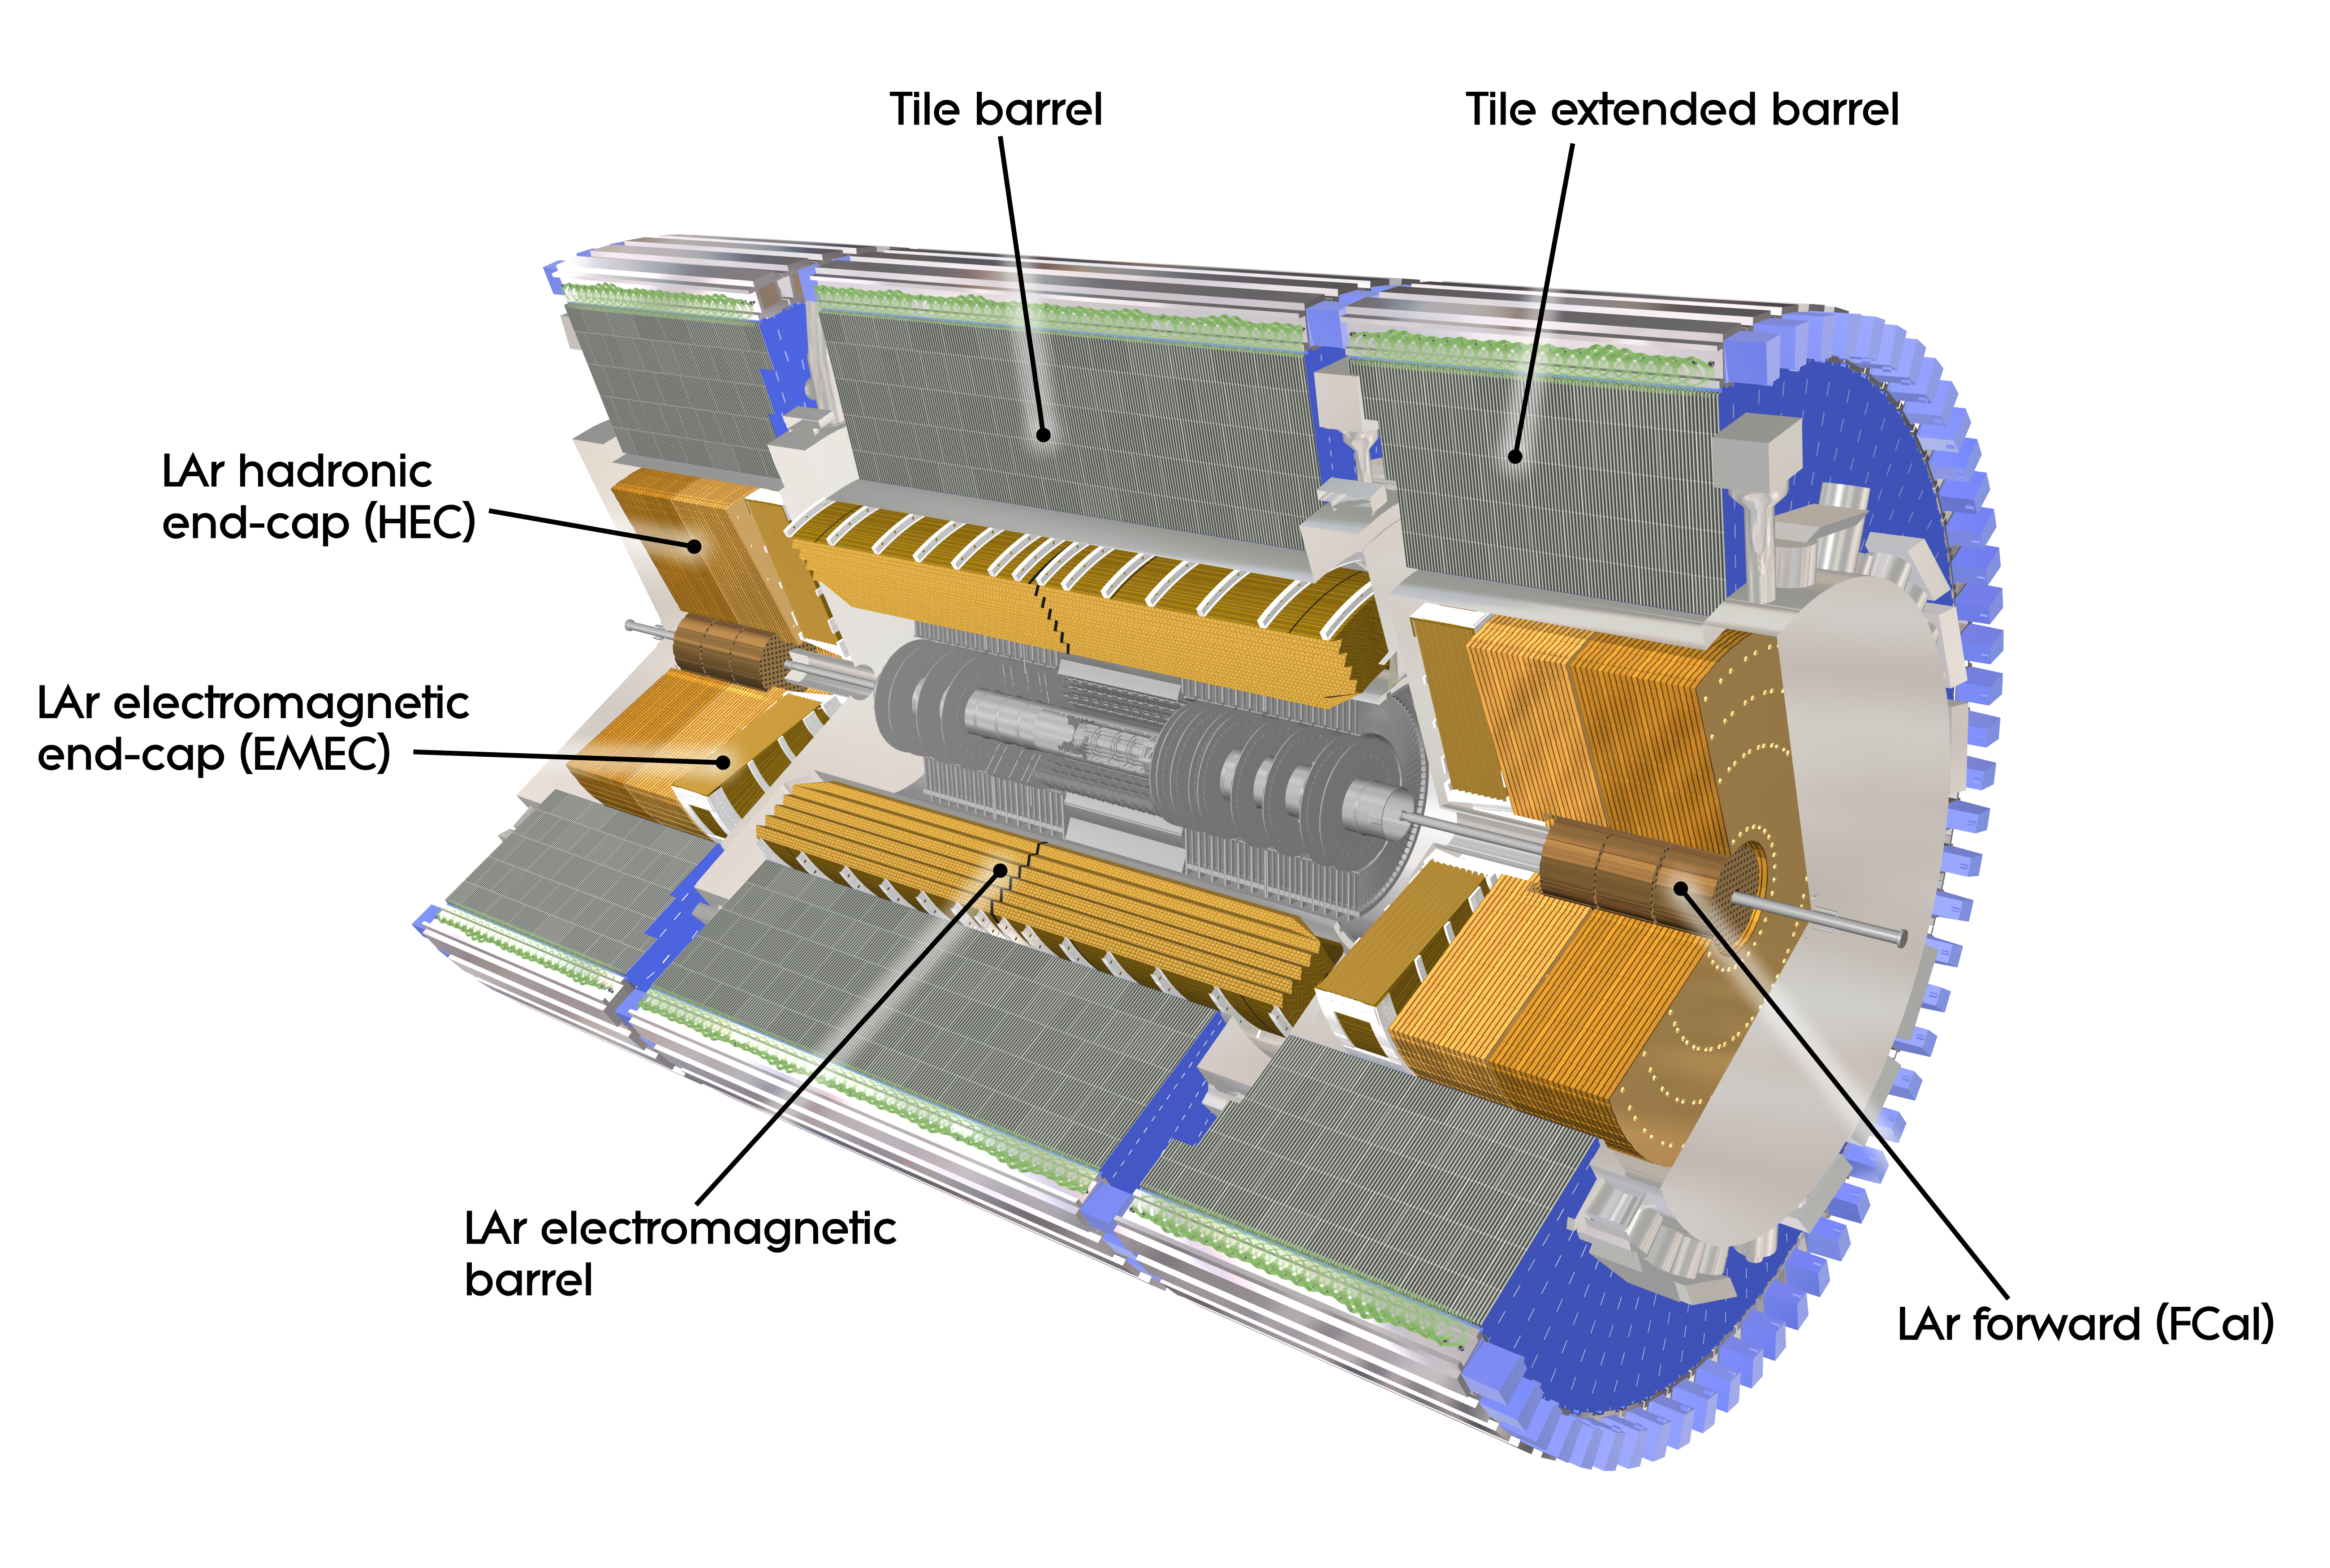
\includegraphics[width=\textwidth]{imagens/calorimetros.jpg}
\caption{Os diversos calorimetros do ATLAS. Extraido de
\cite{muons_images}.}
\label{fig:espec_muons}
\end{figure}

\subsection{O Espectômetro de Mûons}
\label{ssec:espectometro_muons}

\newacronym[type=Abrev]{mdt}{MDT}{Câmaras de Tubos de Movimento Monitorados}
\newacronym[type=Abrev]{csc}{CSC}{Câmaras de Tiras Catódicas}
\newacronym[type=Abrev]{rpc}{RPC}{Câmaras de Chapas Resistivas}
\newacronym[type=Abrev]{tgc}{TGC}{Câmaras de Brechas Finas}

\begin{figure}[h!t]
\centering
\includegraphics[width=0.8\textwidth]{imagens/espectometro_muons_lowres.jpg}
\caption{O Espectômetro de Mûons e seus componentes. Extraido de
\cite{muons_images}.}
\label{fig:espec_muons}
\end{figure}

Os mûons como estados finais são muito importantes em diversas análises e provêm
assinaturas físicas robustas no \gls{lhc}. 
Eles penetram grandes quantidades de material quando a maior parte das outras
partículas são absorvidas, e com o objetivo de medir sua energia, o Espectômetro
de Mûons \cite{muon_tdr} é o subdetector mais externo do \gls{atlas}. Diferente dos calorimetros
que emprega um processo de medição destrutivo, o Espectômetro de Mûons,
Figura~\ref{fig:espec_muons}, mede a carga e o momento de mûons através 
da reconstrução de suas trajetórias no 
campo magnético dos toróides de núcleo a ar de forma semelhante ao \gls{id}. 

As câmaras no barril formam três cilindros
concêntricos com o eixo dos feixes e cobrem um alcance em $|\gls{eta}| < 1$,
estando localizadas a uma distância radial de $\sim$5, 7,5, e 10m. São
utilizados quatro discos para as câmaras da tampa que cobrem um o alcance de 
$1 < |\gls{eta}| < 2,7$ em distâncias de $\sim$7, 10, 14 e 21-23 m do ponto de
interação, todos concêntricos ao tubo do feixe. Deseja-se medir mûons
na região de poucos GeV com uma resolução de $\sim1\%$, enquanto mûons na
faixa de 1 TeV a precisão pode ser um pouco menor, $ < 10\%$. O poder de
curvatura $Bl^2$ fornecido pelos toróides e tamanho do detector é de cerca de 36
$\text{Tm}^2$, comparado com os 2 $\text{Tm}^2$ no \gls{id}. Para fornecer a
resolução de momento desejada a \gls{respos} deve ser de no mínimo
50 $\mu$m em z e 0,5 mrad em R$\phi$ \cite{ATLAS_TDR}.

Existem diversos tipos de câmaras de traços de mûons: As \gls{mdt} e \gls{csc}
são as câmaras de precisão, já as \gls{rpc} e \gls{tgc} são câmaras
rápidas para o \glslink{l1}{Primeiro Nível de filtragem (L1)}. O príncipio de leitura é o mesmo para os quatro
tipos, onde os mûons que passam por uma fenda de gás entre um anôdo e catodo (por
exemplo, um cabo dentro de um tubo ou duas chapas paralelas) causam uma discarga
local no gás sendo assim possível ler o sinal. No total existem 5376 câmaras
com 1,0757 M canais de leitura \cite{tese_jatos}.

Os \glspl{mdt} fornecem medições de precião (acurácia mecânica de 30 $\mu$m) 
dos pontos do traço com 80 $\mu$m de \gls{respos}
para cada cabo em uma larga região de \gls{eta}. Em grandes \gls{eta} e próximo
do ponto de interação são utilizados os \glspl{csc}, que têm uma maior
granularidade e suportam a sua alta demanda causada pelas condições de ruído
físico.
 
As câmaras de filtragem tem uma resolução de tempo menor que o espaçamento
mínimo entre pacotes de 25 ns para fazer possível sua identificação. Os
requerimentos de tempo e espaço são atendidos de acordo com a seguinte
especificação: os \glspl{rpc} têm boa resolução de tempo (1,5 ns), por outro
lado os \glspl{tgc} tem melhor resolução espacial 
(o afastamento entre os cabos anôdos é de 1,8 mm).

Graças a grande dimensão do Espectômetro de Mûon não é possível de firmar as
dimensões e posições das câmaras no nível requerido de 30 $\mu$m. Portanto, as
deformações e posições da câmara são constantemente monitoradas por meio de
sistemas opticos de alinhamento, de forma que deslocamentos dentre $\approx$ 30
$\mu$m e $\approx$ 1 cm podem ser corrigidos em análise pelos algoritmos do
Sistema de Reconstrução \cite{muon_tdr}.

\section{Ferramentas Utilizadas na Colaboração}
\label{sec:ferramentas}

